%\SweaveUTF8
\documentclass[aspectratio=43]{beamer}

\usetheme{default}
% Slide setup, colour independent

\usepackage{amsmath,amssymb,amsthm}
\usepackage[utf8]{inputenc}
\usepackage{colortbl}
\usepackage{bm}
\usepackage{xcolor}
\usepackage{dsfont}
\usepackage{setspace}
%\usepackage{subfigure}
% To use \ding{234} and the like
\usepackage{pifont}
% To cross reference between slide files
\usepackage{zref-xr,zref-user}
% Use something like
% \zexternaldocument{fileI}
% in the tex files. And cite using \zref instead of \ref

% Fields and the like
\def\IC{\mathbb{C}}
\def\IF{\mathbb{F}}
\def\II{\mathbb{I}}
\def\IJ{\mathbb{J}}
\def\IM{\mathbb{M}}
\def\IN{\mathbb{N}}
\def\IP{\mathbb{P}}
\def\IR{\mathbb{R}}
\def\IZ{\mathbb{Z}}
\def\11{\mathds{1}}


% Bold lowercase
\def\ba{\mathbf{a}}
\def\bb{\mathbf{b}}
\def\bc{\mathbf{c}}
\def\bd{\mathbf{d}}
\def\be{\mathbf{e}}
\def\bf{\mathbf{f}}
\def\bh{\mathbf{h}}
\def\bi{\mathbf{i}}
\def\bj{\mathbf{j}}
\def\bk{\mathbf{k}}
\def\bn{\mathbf{n}}
\def\bp{\mathbf{p}}
\def\br{\mathbf{r}}
\def\bs{\mathbf{s}}
\def\bu{\mathbf{u}}
\def\bv{\mathbf{v}}
\def\bw{\mathbf{w}}
\def\bx{\mathbf{x}}
\def\by{\mathbf{y}}
\def\bz{\mathbf{z}}

% Bold capitals
\def\bB{\mathbf{B}}
\def\bD{\mathbf{D}}
\def\bE{\mathbf{E}}
\def\bF{\mathbf{F}}
\def\bG{\mathbf{G}}
\def\bI{\mathbf{I}}
\def\bL{\mathbf{L}}
\def\bN{\mathbf{N}}
\def\bP{\mathbf{P}}
\def\bR{\mathbf{R}}
\def\bS{\mathbf{S}}
\def\bT{\mathbf{T}}
\def\bX{\mathbf{X}}

% Bold numbers
\def\b0{\mathbf{0}}

% Bold greek
\bmdefine{\bmu}{\bm{\mu}}
\def\bphi{\bm{\phi}}
\def\bvarphi{\bm{\varphi}}
\def\bPi{\bm{\Pi}}
\def\bGamma{\bm{\Gamma}}

% Bold red sentence
\def\boldred#1{{\color{red}\textbf{#1}}}
\def\defword#1{{\color{orange}\textbf{#1}}}

% Caligraphic letters
\def\A{\mathcal{A}}
\def\B{\mathcal{B}}
\def\C{\mathcal{C}}
\def\D{\mathcal{D}}
\def\E{\mathcal{E}}
\def\F{\mathcal{F}}
\def\G{\mathcal{G}}
\def\H{\mathcal{H}}
\def\I{\mathcal{I}}
\def\L{\mathcal{L}}
\def\M{\mathcal{M}}
\def\N{\mathcal{N}}
\def\P{\mathcal{P}}
\def\R{\mathcal{R}}
\def\S{\mathcal{S}}
\def\T{\mathcal{T}}
\def\U{\mathcal{U}}
\def\V{\mathcal{V}}

% tt font for code
\def\code#1{{\tt #1}}

% i.e., e.g.
\def\eg{\emph{e.g.}}
\def\ie{\emph{i.e.}}


% Operators and special symbols
\def\nbOne{{\mathchoice {\rm 1\mskip-4mu l} {\rm 1\mskip-4mu l}
{\rm 1\mskip-4.5mu l} {\rm 1\mskip-5mu l}}}
\def\cov{\ensuremath{\mathsf{cov}}}
\def\Var{\ensuremath{\mathsf{Var}\ }}
\def\Im{\textrm{Im}\;}
\def\Re{\textrm{Re}\;}
\def\det{\ensuremath{\mathsf{det}}}
\def\diag{\ensuremath{\mathsf{diag}}}
\def\nullspace{\ensuremath{\mathsf{null}}}
\def\nullity{\ensuremath{\mathsf{nullity}}}
\def\rank{\ensuremath{\mathsf{rank}}}
\def\range{\ensuremath{\mathsf{range}}}
\def\sgn{\ensuremath{\mathsf{sgn}}}
\def\Span{\ensuremath{\mathsf{span}}}
\def\tr{\ensuremath{\mathsf{tr}}}
\def\imply{$\Rightarrow$}
\def\restrictTo#1#2{\left.#1\right|_{#2}}
\newcommand{\parallelsum}{\mathbin{\!/\mkern-5mu/\!}}
\def\dsum{\mathop{\displaystyle \sum }}%
\def\dind#1#2{_{\substack{#1\\ #2}}}

\DeclareMathOperator{\GL}{GL}
\DeclareMathOperator{\Rel}{Re}
\def\Nt#1{\left|\!\left|\!\left|#1\right|\!\right|\!\right|}
\newcommand{\tripbar}{|\! |\! |}



% The beamer bullet (in base colour)
\def\bbullet{\leavevmode\usebeamertemplate{itemize item}\ }

% Theorems and the like
\newtheorem{proposition}[theorem]{Proposition}
\newtheorem{property}[theorem]{Property}
\newtheorem{importantproperty}[theorem]{Property}
\newtheorem{importanttheorem}[theorem]{Theorem}
%\newtheorem{lemma}[theorem]{Lemma}
%\newtheorem{corollary}[theorem]{Corollary}
\newtheorem{remark}[theorem]{Remark}
\setbeamertemplate{theorems}[numbered]
%\setbeamertemplate{theorems}[ams style]

%
%\usecolortheme{orchid}
%\usecolortheme{orchid}

\def\red{\color[rgb]{1,0,0}}
\def\blue{\color[rgb]{0,0,1}}
\def\green{\color[rgb]{0,1,0}}


% Get rid of navigation stuff
\setbeamertemplate{navigation symbols}{}

% Set footline/header line
\setbeamertemplate{footline}
{%
\quad p. \insertpagenumber \quad--\quad \insertsection\vskip2pt
}
% \setbeamertemplate{headline}
% {%
% \quad\insertsection\hfill p. \insertpagenumber\quad\mbox{}\vskip2pt
% }


\makeatletter
\newlength\beamerleftmargin
\setlength\beamerleftmargin{\Gm@lmargin}
\makeatother

% Colours for special pages
\def\extraContent{yellow!20}


%%%%%%%%%%%%%%%%%
\usepackage{tikz}
\usetikzlibrary{shapes,arrows}
\usetikzlibrary{positioning}
\usetikzlibrary{shapes.symbols,shapes.callouts,patterns}
\usetikzlibrary{calc,fit}
\usetikzlibrary{backgrounds}
\usetikzlibrary{decorations.pathmorphing,fit,petri}
\usetikzlibrary{automata}
\usetikzlibrary{fadings}
\usetikzlibrary{patterns,hobby}

\usetikzlibrary{backgrounds,fit,petri}


\usepackage{pgfplots}
\pgfplotsset{compat=1.6}
\pgfplotsset{ticks=none}

\usetikzlibrary{decorations.markings}
\usetikzlibrary{arrows.meta}
\tikzset{>=stealth}

% For tikz
\usetikzlibrary{shapes,arrows}
\usetikzlibrary{positioning}
\tikzstyle{cloud} = [draw, ellipse,fill=red!20, node distance=0.87cm,
minimum height=2em]
\tikzstyle{line} = [draw, -latex']


%%% For max frame images
\newenvironment{changemargin}[2]{%
\begin{list}{}{%
\setlength{\topsep}{0pt}%
\setlength{\leftmargin}{#1}%
\setlength{\rightmargin}{#2}%
\setlength{\listparindent}{\parindent}%
\setlength{\itemindent}{\parindent}%
\setlength{\parsep}{\parskip}%
}%
\item[]}{\end{list}}


% Make one image take up the entire slide content area in beamer,.:
% centered/centred full-screen image, with title:
% This uses the whole screen except for the 1cm border around it
% all. 128x96mm
\newcommand{\titledFrameImage}[2]{
\begin{frame}{#1}
%\begin{changemargin}{-1cm}{-1cm}
\begin{center}
\includegraphics[width=108mm,height=\textheight,keepaspectratio]{#2}
\end{center}
%\end{changemargin}
\end{frame}
}

% Make one image take up the entire slide content area in beamer.:
% centered/centred full-screen image, no title:
% This uses the whole screen except for the 1cm border around it
% all. 128x96mm
\newcommand{\plainFrameImage}[1]{
\begin{frame}[plain]
%\begin{changemargin}{-1cm}{-1cm}
\begin{center}
\includegraphics[width=108mm,height=76mm,keepaspectratio]{#1}
\end{center}
%\end{changemargin}
\end{frame}
}

% Make one image take up the entire slide area, including borders, in beamer.:
% centered/centred full-screen image, no title:
% This uses the entire whole screen
\newcommand{\maxFrameImage}[1]{
\begin{frame}[plain]
\begin{changemargin}{-1cm}{-1cm}
\begin{center}
\includegraphics[width=\paperwidth,height=\paperheight,keepaspectratio]
{#1}
\end{center}
\end{changemargin}
\end{frame}
}

% This uses the entire whole screen (to include in frame)
\newcommand{\maxFrameImageNoFrame}[1]{
\begin{changemargin}{-1cm}{-1cm}
\begin{center}
\includegraphics[width=\paperwidth,height=0.99\paperheight,keepaspectratio]
{#1}
\end{center}
\end{changemargin}
}

% Make one image take up the entire slide area, including borders, in beamer.:
% centered/centred full-screen image, no title:
% This uses the entire whole screen
\newcommand{\maxFrameImageColor}[2]{
\begin{frame}[plain]
\setbeamercolor{normal text}{bg=#2!20}
\begin{changemargin}{-1cm}{-1cm}
\begin{center}
\includegraphics[width=\paperwidth,height=\paperheight,keepaspectratio]
{#1}
\end{center}
\end{changemargin}
\end{frame}
}


\usepackage{tikz}
\usetikzlibrary{patterns,hobby}
\usepackage{pgfplots}
\pgfplotsset{compat=1.6}
\pgfplotsset{ticks=none}

\usetikzlibrary{backgrounds}
\usetikzlibrary{decorations.markings}
\usetikzlibrary{arrows.meta}
\tikzset{>=stealth}

\tikzset{
  clockwise arrows/.style={
    postaction={
      decorate,
      decoration={
        markings,
        mark=between positions 0.1 and 0.9 step 40pt with {\arrow{>}},
   }}}}


   %%%%%%%%%%%
% To have links to parts in the outline
\makeatletter
\AtBeginPart{%
  \addtocontents{toc}{\protect\beamer@partintoc{\the\c@part}{\beamer@partnameshort}{\the\c@page}}%
}
%% number, shortname, page.
\providecommand\beamer@partintoc[3]{%
  \ifnum\c@tocdepth=-1\relax
    % requesting onlyparts.
    \makebox[6em]{Part #1:} \textcolor{green!30!blue}{\hyperlink{#2}{#2}}
    \par
  \fi
}
\define@key{beamertoc}{onlyparts}[]{%
  \c@tocdepth=-1\relax
}
\makeatother%

\newcommand{\nameofthepart}{}
\newcommand{\nupart}[1]%
    {   \part{#1}%
        \renewcommand{\nameofthepart}{#1}%
        {
          \setbeamercolor{background canvas}{bg=orange!50}
          \begin{frame}{#1}%\partpage 
          \hypertarget{\nameofthepart}{}\tableofcontents%
          \end{frame}
        }
    }



\usecolortheme{orchid}
%% Listings
\usepackage{listings}
\definecolor{mygreen}{rgb}{0,0.6,0}
\definecolor{mygray}{rgb}{0.5,0.5,0.5}
\definecolor{mymauve}{rgb}{0.58,0,0.82}
\definecolor{mygold}{rgb}{1,0.843,0}
\definecolor{myblue}{rgb}{0.537,0.812,0.941}

\definecolor{lgreen}{rgb}{0.6,0.9,.6}
\definecolor{lred}{rgb}{1,0.5,.5}

\lstloadlanguages{R}
\lstset{ %
  language=R,
  backgroundcolor=\color{black!05},   % choose the background color
  basicstyle=\footnotesize\ttfamily,        % size of fonts used for the code
  breaklines=true,                 % automatic line breaking only at whitespace
  captionpos=b,                    % sets the caption-position to bottom
  commentstyle=\color{mygreen},    % comment style
  escapeinside={\%*}{*)},          % if you want to add LaTeX within your code
  keywordstyle=\color{red},       % keyword style
  stringstyle=\color{mygold},     % string literal style
  keepspaces=true,
  columns=fullflexible,
  tabsize=4,
}
% Could also do (in lstset)
% basicstyle==\fontfamily{pcr}\footnotesize
\lstdefinelanguage{Renhanced}%
  {keywords={abbreviate,abline,abs,acos,acosh,action,add1,add,%
      aggregate,alias,Alias,alist,all,anova,any,aov,aperm,append,apply,%
      approx,approxfun,apropos,Arg,args,array,arrows,as,asin,asinh,%
      atan,atan2,atanh,attach,attr,attributes,autoload,autoloader,ave,%
      axis,backsolve,barplot,basename,besselI,besselJ,besselK,besselY,%
      beta,binomial,body,box,boxplot,break,browser,bug,builtins,bxp,by,%
      c,C,call,Call,case,cat,category,cbind,ceiling,character,char,%
      charmatch,check,chol,chol2inv,choose,chull,class,close,cm,codes,%
      coef,coefficients,co,col,colnames,colors,colours,commandArgs,%
      comment,complete,complex,conflicts,Conj,contents,contour,%
      contrasts,contr,control,helmert,contrib,convolve,cooks,coords,%
      distance,coplot,cor,cos,cosh,count,fields,cov,covratio,wt,CRAN,%
      create,crossprod,cummax,cummin,cumprod,cumsum,curve,cut,cycle,D,%
      data,dataentry,date,dbeta,dbinom,dcauchy,dchisq,de,debug,%
      debugger,Defunct,default,delay,delete,deltat,demo,de,density,%
      deparse,dependencies,Deprecated,deriv,description,detach,%
      dev2bitmap,dev,cur,deviance,off,prev,,dexp,df,dfbetas,dffits,%
      dgamma,dgeom,dget,dhyper,diag,diff,digamma,dim,dimnames,dir,%
      dirname,dlnorm,dlogis,dnbinom,dnchisq,dnorm,do,dotplot,double,%
      download,dpois,dput,drop,drop1,dsignrank,dt,dummy,dump,dunif,%
      duplicated,dweibull,dwilcox,dyn,edit,eff,effects,eigen,else,%
      emacs,end,environment,env,erase,eval,equal,evalq,example,exists,%
      exit,exp,expand,expression,External,extract,extractAIC,factor,%
      fail,family,fft,file,filled,find,fitted,fivenum,fix,floor,for,%
      For,formals,format,formatC,formula,Fortran,forwardsolve,frame,%
      frequency,ftable,ftable2table,function,gamma,Gamma,gammaCody,%
      gaussian,gc,gcinfo,gctorture,get,getenv,geterrmessage,getOption,%
      getwd,gl,glm,globalenv,gnome,GNOME,graphics,gray,grep,grey,grid,%
      gsub,hasTsp,hat,heat,help,hist,home,hsv,httpclient,I,identify,if,%
      ifelse,Im,image,\%in\%,index,influence,measures,inherits,install,%
      installed,integer,interaction,interactive,Internal,intersect,%
      inverse,invisible,IQR,is,jitter,kappa,kronecker,labels,lapply,%
      layout,lbeta,lchoose,lcm,legend,length,levels,lgamma,library,%
      licence,license,lines,list,lm,load,local,locator,log,log10,log1p,%
      log2,logical,loglin,lower,lowess,ls,lsfit,lsf,ls,machine,Machine,%
      mad,mahalanobis,make,link,margin,match,Math,matlines,mat,matplot,%
      matpoints,matrix,max,mean,median,memory,menu,merge,methods,min,%
      missing,Mod,mode,model,response,mosaicplot,mtext,mvfft,na,nan,%
      names,omit,nargs,nchar,ncol,NCOL,new,next,NextMethod,nextn,%
      nlevels,nlm,noquote,NotYetImplemented,NotYetUsed,nrow,NROW,null,%
      numeric,\%o\%,objects,offset,old,on,Ops,optim,optimise,optimize,%
      options,or,order,ordered,outer,package,packages,page,pairlist,%
      pairs,palette,panel,par,parent,parse,paste,path,pbeta,pbinom,%
      pcauchy,pchisq,pentagamma,persp,pexp,pf,pgamma,pgeom,phyper,pico,%
      pictex,piechart,Platform,plnorm,plogis,plot,pmatch,pmax,pmin,%
      pnbinom,pnchisq,pnorm,points,poisson,poly,polygon,polyroot,pos,%
      postscript,power,ppoints,ppois,predict,preplot,pretty,Primitive,%
      print,prmatrix,proc,prod,profile,proj,prompt,prop,provide,%
      psignrank,ps,pt,ptukey,punif,pweibull,pwilcox,q,qbeta,qbinom,%
      qcauchy,qchisq,qexp,qf,qgamma,qgeom,qhyper,qlnorm,qlogis,qnbinom,%
      qnchisq,qnorm,qpois,qqline,qqnorm,qqplot,qr,Q,qty,qy,qsignrank,%
      qt,qtukey,quantile,quasi,quit,qunif,quote,qweibull,qwilcox,%
      rainbow,range,rank,rbeta,rbind,rbinom,rcauchy,rchisq,Re,read,csv,%
      csv2,fwf,readline,socket,real,Recall,rect,reformulate,regexpr,%
      relevel,remove,rep,repeat,replace,replications,report,require,%
      resid,residuals,restart,return,rev,rexp,rf,rgamma,rgb,rgeom,R,%
      rhyper,rle,rlnorm,rlogis,rm,rnbinom,RNGkind,rnorm,round,row,%
      rownames,rowsum,rpois,rsignrank,rstandard,rstudent,rt,rug,runif,%
      rweibull,rwilcox,sample,sapply,save,scale,scan,scan,screen,sd,se,%
      search,searchpaths,segments,seq,sequence,setdiff,setequal,set,%
      setwd,show,sign,signif,sin,single,sinh,sink,solve,sort,source,%
      spline,splinefun,split,sqrt,stars,start,stat,stem,step,stop,%
      storage,strstrheight,stripplot,strsplit,structure,strwidth,sub,%
      subset,substitute,substr,substring,sum,summary,sunflowerplot,svd,%
      sweep,switch,symbol,symbols,symnum,sys,status,system,t,table,%
      tabulate,tan,tanh,tapply,tempfile,terms,terrain,tetragamma,text,%
      time,title,topo,trace,traceback,transform,tri,trigamma,trunc,try,%
      ts,tsp,typeof,unclass,undebug,undoc,union,unique,uniroot,unix,%
      unlink,unlist,unname,untrace,update,upper,url,UseMethod,var,%
      variable,vector,Version,vi,warning,warnings,weighted,weights,%
      which,while,window,write,\%x\%,x11,X11,xedit,xemacs,xinch,xor,%
      xpdrows,xy,xyinch,yinch,zapsmall,zip},%
   otherkeywords={!,!=,~,$,*,\%,\&,\%/\%,\%*\%,\%\%,<-,<<-,_,/},%
   alsoother={._$},%
   sensitive,%
   morecomment=[l]\#,%
   morestring=[d]",%
   morestring=[d]'% 2001 Robert Denham
  }%

%%%%%%% 
%% Definitions in yellow boxes
\usepackage{etoolbox}
\setbeamercolor{block title}{use=structure,fg=structure.fg,bg=structure.fg!40!bg}
\setbeamercolor{block body}{parent=normal text,use=block title,bg=block title.bg!20!bg}

\BeforeBeginEnvironment{definition}{%
	\setbeamercolor{block title}{fg=black,bg=yellow!20!white}
	\setbeamercolor{block body}{fg=black, bg=yellow!05!white}
}
\AfterEndEnvironment{definition}{
	\setbeamercolor{block title}{use=structure,fg=structure.fg,bg=structure.fg!20!bg}
	\setbeamercolor{block body}{parent=normal text,use=block title,bg=block title.bg!50!bg, fg=black}
}
\BeforeBeginEnvironment{importanttheorem}{%
	\setbeamercolor{block title}{fg=black,bg=red!20!white}
	\setbeamercolor{block body}{fg=black, bg=red!05!white}
}
\AfterEndEnvironment{importanttheorem}{
	\setbeamercolor{block title}{use=structure,fg=structure.fg,bg=structure.fg!20!bg}
	\setbeamercolor{block body}{parent=normal text,use=block title,bg=block title.bg!50!bg, fg=black}
}
\BeforeBeginEnvironment{importantproperty}{%
	\setbeamercolor{block title}{fg=black,bg=red!50!white}
	\setbeamercolor{block body}{fg=black, bg=red!30!white}
}
\AfterEndEnvironment{importantproperty}{
	\setbeamercolor{block title}{use=structure,fg=structure.fg,bg=structure.fg!20!bg}
	\setbeamercolor{block body}{parent=normal text,use=block title,bg=block title.bg!50!bg, fg=black}
}

% Colour for the outline page
\definecolor{outline_colour}{RGB}{230,165,83}
%% Colours for sections, subsections aand subsubsections
\definecolor{section_colour}{RGB}{27,46,28}
\definecolor{subsection_colour}{RGB}{52,128,56}
\definecolor{subsubsection_colour}{RGB}{150,224,154}
% Beginning of a section
\AtBeginSection[]{
	{
		\setbeamercolor{background canvas}{bg=section_colour}
		\begin{frame}[noframenumbering,plain]
			\framesubtitle{\nameofthepart Chapter \insertromanpartnumber \ -- \iteminsert{\insertpart}}
			\tableofcontents[
				currentsection,
				sectionstyle=show/shaded,
				subsectionstyle=show/hide/hide,
				subsubsectionstyle=hide/hide/hide]
		\end{frame}
	\addtocounter{page}{-1}
	%\addtocounter{framenumber}{-1} 
	}
}

% Beginning of a section
\AtBeginSubsection[]{
	{
		\setbeamercolor{background canvas}{bg=subsection_colour}
		\begin{frame}[noframenumbering,plain]
				\framesubtitle{\nameofthepart Chapter \insertromanpartnumber \ -- \iteminsert{\insertpart}}
				\tableofcontents[
					currentsection,
					sectionstyle=show/hide,
					currentsubsection,
					subsectionstyle=show/shaded/hide,
					subsubsectionstyle=show/hide/hide]
			\end{frame}
		\addtocounter{page}{-1}
	}
}

% Beginning of a section
\AtBeginSubsubsection[]{
	{
		\setbeamercolor{background canvas}{bg=subsubsection_colour}
		\begin{frame}[noframenumbering,plain]
				\framesubtitle{\nameofthepart Chapter \insertromanpartnumber \ -- \iteminsert{\insertpart}}
				\tableofcontents[
					currentsection,
					sectionstyle=show/hide,
					subsectionstyle=show/shaded/hide]
					%currentsubsubsection]
			\end{frame}
		\addtocounter{page}{-1}
	}
}


\title{Introduction to mathematical epidemiology}
\subtitle{Lecture 01}
\author{Julien Arino}
\date{September 2023}

\usepackage{Sweave}
\begin{document}



% The title page
\begin{frame}[noframenumbering,plain]
  \titlepage
\end{frame}
\addtocounter{page}{-1}

\begin{frame}
    \tableofcontents[hideallsubsections]
\end{frame}
\addtocounter{page}{-1}

%%%%%%%%%%%%%%%%%%%
%%%%%%%%%%%%%%%%%%%
%%%%%%%%%%%%%%%%%%%
%%%%%%%%%%%%%%%%%%%
%%%%%%%%%%%%%%%%%%%
%%%%%%%%%%%%%%%%%%%
%%%%%%%%%%%%%%%%%%%
%%%%%%%%%%%%%%%%%%%
\section{Epidemics}

%%%%%%%%%%%%%%%%%%%%
%%%%%%%%%%%%%%%%%%%%
\subsection{General historical remarks}
\begin{frame}{Among the first events recorded}
- Epidemic events are among the first events recorded in History
\vfill
- Indeed their effect was devastating at a time when medicine virtually did not exist and thus easily observed
\end{frame}

\begin{frame}{First known epidemics (\href{https://en.wikipedia.org/wiki/List_of_epidemics}{from Wikipedia})}

% | Event | Date | Location | Disease | Death toll (estimate) |
% |---|---|---|---|---|
% | Plague of Megiddo | 1350 BCE | Megiddo, land of Canaan | Unknown | Unknown | 
% | [Plague of Athens](https://en.wikipedia.org/wiki/Plague_of_Athens) | 429–426 BCE | Greece, Libya, Egypt, Ethiopia | Possibly typhus, typhoid fever or VHF |  75,000–100,000 |
% | [412 BCE epidemic](https://en.wikipedia.org/wiki/412_BC_epidemic) |412 BCE | Greece, Roman Republic | Possibly influenza | Unknown |
% | [Antonine Plague](https://en.wikipedia.org/wiki/Antonine_Plague) | 165–180 CE (possibly up to 190 CE) | Roman Empire | Possibly smallpox | 5–10 million |
% | Jian'an Plague | 217 CE | Han dynasty | Possibly typhoid fever or VHF | Unknown |
% | [Plague of Cyprian](https://en.wikipedia.org/wiki/Plague_of_Cyprian) | 250–266 CE | Europe | Possibly smallpox | Unknown |
% | [Plague of Justinian](https://en.wikipedia.org/wiki/Plague_of_Justinian) (1st plague pandemic) | 541–549 CE | Europe and West Asia | Bubonic plague | 15–100 million (25–60% of population of Europe) | 
% | [Roman Plague of 590](https://en.wikipedia.org/wiki/Roman_Plague_of_590) (1st plague pandemic) | 590 CE | Rome, Byzantine Empire | Bubonic plague | Unknown |
% | [Plague of Sheroe](https://en.wikipedia.org/wiki/Plague_of_Sheroe) (1st plague pandemic) | 627–628 CE | Bilad al-Sham | Bubonic plague | 25,000+ |
% | [Plague of Amwas](https://en.wikipedia.org/wiki/Plague_of_Amwas) (1st plague pandemic) | 638–639 CE | Byzantine Empire, West Asia, Africa | Bubonic plague | 25,000+ |
% | [Plague of 664](https://en.wikipedia.org/wiki/Plague_of_664) (1st plague pandemic)  | 664–689 CE | British Isles | Bubonic plague | Unknown |
% | Plague of 698–701 (1st plague pandemic) | 698–701 CE | Byzantine Empire, West Asia, Syria, Mesopotamia | Bubonic plague |Unknown |
% | [735–737 Japanese smallpox epidemic](https://en.wikipedia.org/wiki/735%E2%80%93737_Japanese_smallpox_epidemic) | 735–737 CE | Japan | Smallpox | 2 million (approx. 1/3 of Japanese population) | 
% | Plague of 746–747 (1st plague pandemic) | 746–747 CE | Byzantine Empire, West Asia, Africa | Bubonic plague |Unknown |
\end{frame}

\begin{frame}{Epidemics with major human cost}

    % | Rang | Épidémie/pandémie | Maladie | Coût humain | Mortalité globale | Mortalité régionale | Date | Lieux |
    % |:\end{frame}
    
    
    % \begin{frame}
    % :|\end{frame}
    
    
    % \begin{frame}
    % |\end{frame}
    
    
    % \begin{frame}
    % |---|---|---|:---:|---|
    % | 1 | Grande peste | Peste bubonique | 75-200 M |17-54% | 30-60% de la population européenne | 1346-1353 | Europe, Asie et Afrique du Nord |
    % | 2 | Grippe espagnole | Influenza A/H1N1 |  17-100 M |1-5.4% | | 1918-1920 | Monde |
    % | 3 | Peste de Justinien | Peste bubonique | 15-100 M |7-56% | 25-60% de la population Européenne | 541-549 |Afrique du Nord, Europe et Asie de l'Est |
    % | 4 | VIH/SIDA | VIH/SIDA | 36.3 M (en 2020) | Changement population totale trop important pour calculer | | 1981-présent | Monde |
    % | 5 | COVID-19 | SARS-CoV-2 | 6.3-25 M (au 21 mai 2022) | 0.1-0.3% || 2019-présent | Monde |
    % | 6 | 3ème pandémie de peste | Peste bubonique | 12-15 M | | | 1855-1960 | Monde |
    % | 7 | Épidémie de Cocoliztli de 1545-1548 | Cocoliztli | 5-15 M | 1-3% | 27-80% de la population du Mexique | 1545-1548 | Mexique |
    % | 8 | Peste Antonine | Variole ou rougeole | 5-10 M | 3-6 | 25-33% de la population Romaine | 165-180 (peut être 190) | Empire Romain |
    % | 9 | Épidémie de variole du Mexique de 1520 | Variole | 5-8 M | 1-2% | 23-37% de la population du Mexique |1519-1520 | Mexique |
    % | 10 | Épidémie de typhus de Russie de 1918-1922 | Typhus | 2-3 M | 0.1-0.16% | 1-1.6% de la population Russe |1918-1922 | URSS |
    % | 11 | Pandémie d'influenza de 1957-1958 | Influenza A/H2N2 | 1-4 M | 0.03–0.1%| | 1957-1958 | Monde |
    % | 12 | Grippe de Hong Kong | Influenza A/H3N2 | 1-4 M | 0.03-0.1% | | 1968-1969 | Monde |
    % | 13 | Épidémie de Cocoliztli de 1576 | Cocoliztli | 2-2.5 M | 0.4-0.5% | 50% de la population du Mexique | 1576-1580 | Mexique |
    % | 14 | Épidémie japonaise de variole de 735-737 | Variole | 2 M | 1% | 33% de la population du Japon | 735-737 | Japon |
    % | 15 | Peste perse de 1772-1773 | Peste bubonique | 2 M | 0.2–0.3% | | 1772-1773 | Perse |
    % | 16 | Peste de Naples (1656) | Peste bubonique | 1.25 M | 0.2% | | 1656-1658 | Sud de l'Italie |
    % | 17 | Pandémie de choléra de 1846-1860 | Choléra | 1+ M | 0.08% | | 1846-1860 | Monde |
    % | 18 | Peste italienne de 1629-1631 | Peste bubonique |1 M | 0.2% | | 1629-1631 | Italie |
    % | 19 | Pandémie de grippe de 1889-1890 |Influenza (en doute) | 1 M | 0.07% | | 1889-1890 | Monde |
    
\end{frame}
    
%%%%%%%%%%%%%%%%%%%%
%%%%%%%%%%%%%%%%%%%%
\subsection{Unfortunately not yet historical}
\begin{frame}{``Forgotten'' killers}
    - Tuberculosis (TB). In 2020, estimated 10 M cases of active TB, leading to 1.5 M deaths
    \vfill
    - Malaria: 229 M cases and 409 000 deaths in 2019
\end{frame}
    
    
\begin{frame}{Neglected tropical diseases (NTD)}
Often endemic diseases, sometimes major causes of death, but out of sight of rich countries. De \href{https://fr.wikipedia.org/wiki/Maladies_tropicales_négligées}{Wikipedia}, sachant que la liste précise varie selon les auteurs :
    
    % <style scoped>
    % table {
    %     height: 100%;
    %     width: 100%;
    %     font-size: 20px;
    % }
    % </style>
    
    % | | | | 
    % |---|---|---|
    % | [Ulcère de Buruli](https://fr.wikipedia.org/wiki/Ulc%C3%A8re_de_Buruli) | [Maladie de Chagas](https://fr.wikipedia.org/wiki/Maladie_de_Chagas) | Dengue & Chikungunya | 
    % | [Dracunculose](https://fr.wikipedia.org/wiki/Dracunculose) | Echinococcosis | Yaws |
    % | Fascioliasis | [Trypanosomiase](https://fr.wikipedia.org/wiki/Maladie_du_sommeil) | [Leishmaniose](https://fr.wikipedia.org/wiki/Leishmaniose) | 
    % | [Lèpre](https://fr.wikipedia.org/wiki/L%C3%A8pre) | [Filariose lymphatique](https://fr.wikipedia.org/wiki/Filariose_de_Bancroft) | Onchocerciasis |
    % | Rabies | Schistosomiasis | Soil-transmitted helminthiasis | 
    % Cysticercosis | Trachoma | Scabies and other ectoparasites |
    % | Snakebite envenoming | Mycetoma and deep mycoses |
\end{frame}

%%%%%%%%%%%%%%%%%%%%
%%%%%%%%%%%%%%%%%%%%
\subsection{A few examples}


\begin{frame}{The Black Death}
\end{frame}

\begin{frame}{The British Plague of 1547}
\end{frame}

\begin{frame}{The Plague of Marseille of 1720}
\end{frame}
%%%%%%%%%%%%%%%%%%%%
%%%%%%%%%%%%%%%%%%%%
%%%%%%%%%%%%%%%%%%%%
%%%%%%%%%%%%%%%%%%%%
\section{Epidemiology}

%%%%%%%%%%%%%%%%%%%%
%%%%%%%%%%%%%%%%%%%%
\subsection{Definition}
\begin{frame}{Definition}

\begin{itemize}
    \item[\href{https://en.wikipedia.org/wiki/Epidemiology}{Wiki}] 
    \defword{Epidemiology} is the study and analysis of the distribution (who, when, and where), patterns and determinants of health and disease conditions in defined populations
    \item[\href{https://www.bmj.com/about-bmj/resources-readers/publications/epidemiology-uninitiated/1-what-epidemiology}{BMJ}]
    \defword{Epidemiology} is the study of how often diseases occur in different groups of people and why. Epidemiological information is used to plan and evaluate strategies to prevent illness and as a guide to the management of patients in whom disease has already developed 
\end{itemize}
\vfill
Etymology: \emph{the study of what is upon the people}, derived from the Greek \emph{epi} (\emph{upon}, \emph{among}), \emph{demos} (\emph{people}, \emph{district}) and \emph{logos} (\emph{study}, \emph{word}, \emph{discourse})
\end{frame}

%%%%%%%%%%%%%%%%%%%%
%%%%%%%%%%%%%%%%%%%%
\subsection{Who, when and where}


\begin{frame}{Who, when and where}
Recall part of the definition on Wikipedia
\begin{quote}
\defword{Epidemiology} is the study and analysis of the distribution (who, when, and where)  
\end{quote}
\end{frame}


\begin{frame}{A terminologically heavy domain}
A few pointers:
\vfill
- Moghadas and Laskowski. \href{https://nccid.ca/wp-content/uploads/sites/2/2015/03/ReviewTermsFluWEB.pdf}{Review of terms used in modelling influenza infection}. NCCID 2014
\vfill
- Milwid et al. \href{https://doi.org/10.3389/fpubh.2016.00213}{Toward standardizing a lexicon of infectious disease modeling terms}. Frontiers in Public Health 2016
\end{frame}


\begin{frame}{Who}
- \defword{Epidemiology} typically used when dealing with humans, but sometimes also generically when an easy description is sought; e.g., plant disease epidemiology
\vfill
- \defword{Epizootic}: denoting or relating to a disease that is temporarily prevalent and widespread in an animal population
\vfill
- \defword{Panzootic} is like a pandemic for animals
\vfill
- \defword{One Health}: considers health of humans, animals and their environment (including plants)
\end{frame}


\begin{frame}
    \centering
    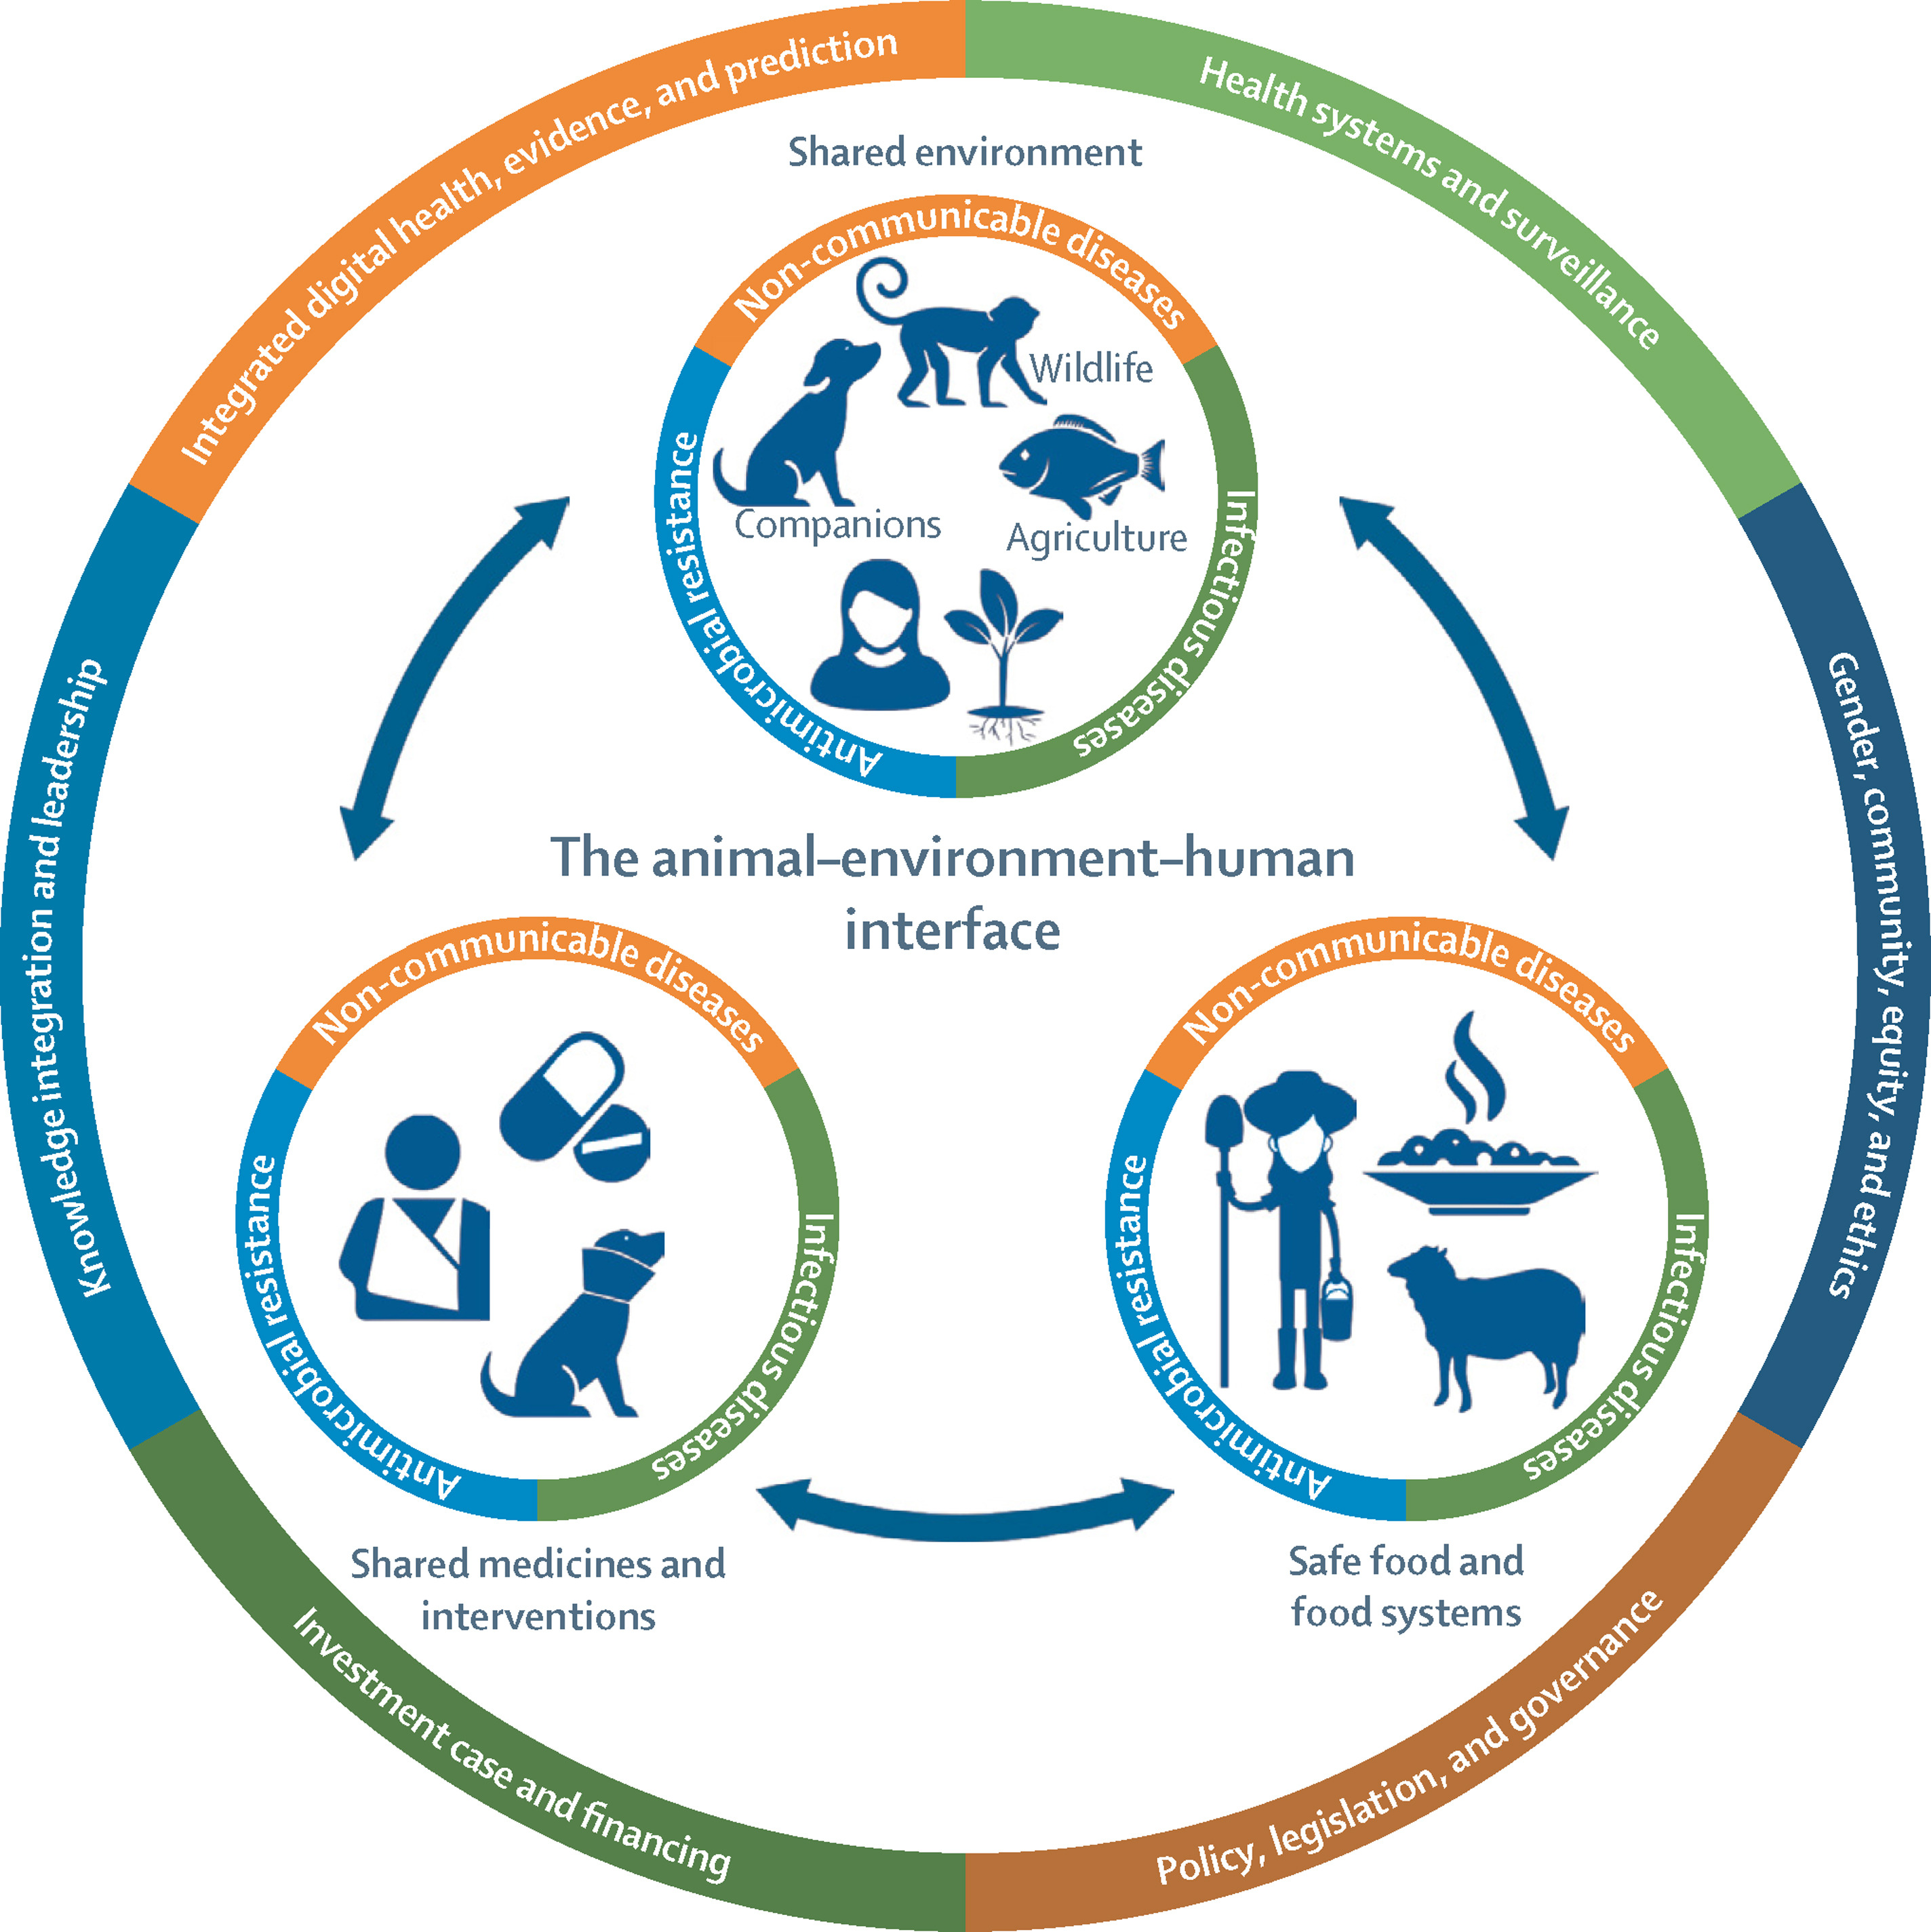
\includegraphics[height=\textheight]{FIGS/gr1_lrg.jpg}
% "https://doi.org/10.1016/S0140-6736(20)31027-8"
\end{frame}


\begin{frame}{Incidence \& Prevalence (when?)}
\defword{Incidence}: number of new cases in a population generated within a certain time period
\vfill
\defword{Prevalence}: number of cases of a disease at a single time point in a population
\vfill
$\implies$ $I(t)$ in an epidemiological model is \textbf{prevalence}, not \textbf{incidence}
\end{frame}

\begin{frame}{Exposition versus Exposed}
- Some bright bulb (not sure who) in days of yore: let's call \textbf{exposed} someone who has contracted the disease but is not yet showing symptoms ($\implies$ SEIR model)
\vfill
- "Real" epidemiologist: let's trace people who were exposed to the virus, i.e., people having come into contact with the virus (whether they have contracted the disease or not)
\vfill
- Interestingly, I have embarked on a quixotic quest to make people use $L$ instead of $E$, only to be told by real epidemiologists that they don't care \code{:)}
\end{frame}


\begin{frame}{The different stages of propagation}
        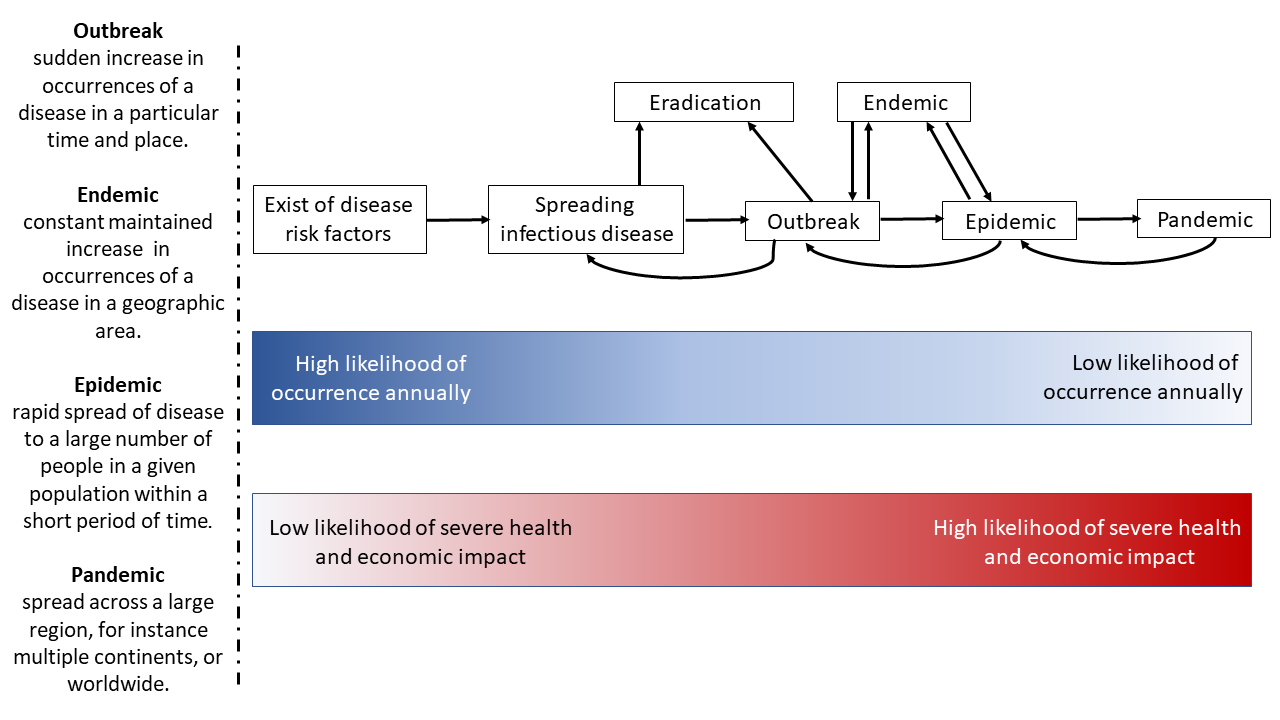
\includegraphics[width=\textwidth]{FIGS/Difference_between_outbreak,_endemic,_epidemic_and_pandemic-en.png}
\end{frame}
        


\begin{frame}{Epidemic curves}
- Used to record the occurrence of new cases as a function of time
\vfill
- When not too many cases, usually "individualised" (bar plots)
\vfill
- When number of cases is large, continuous curve
\end{frame}


\begin{frame}
    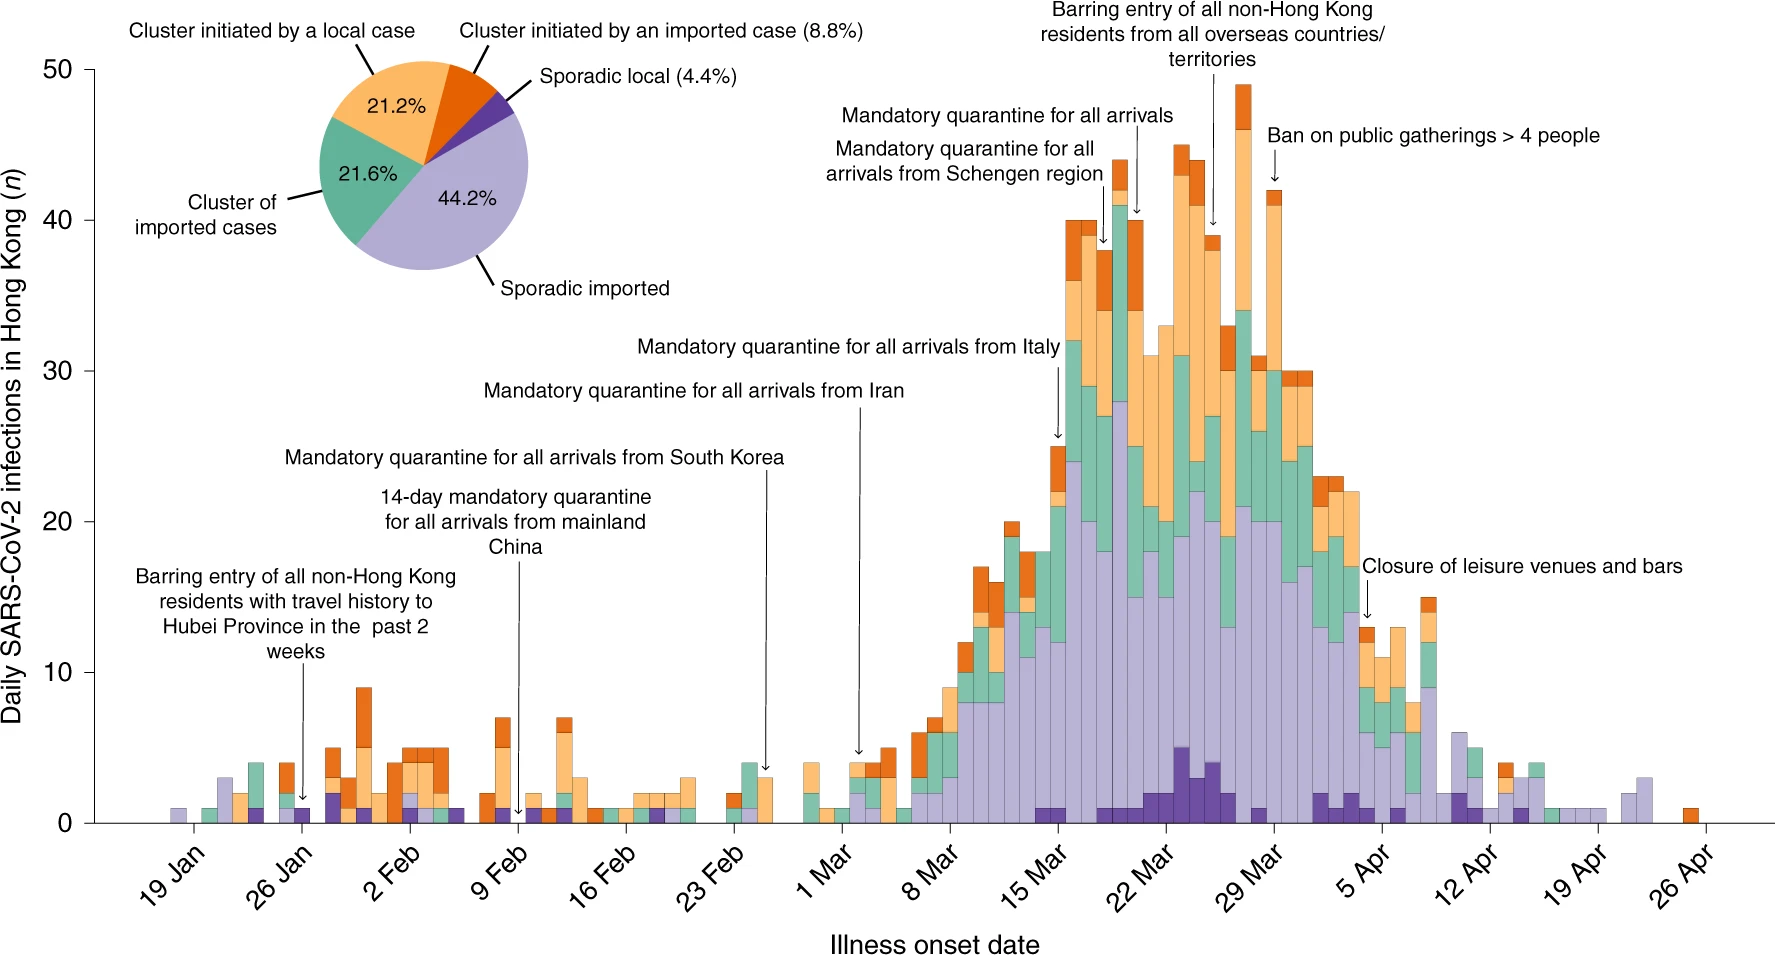
\includegraphics[width=\textwidth]{FIGS/41591_2020_1092_Fig1_HTML.png}
%"https://doi.org/10.1038/s41591-020-1092-0"
\end{frame}


\begin{frame}
    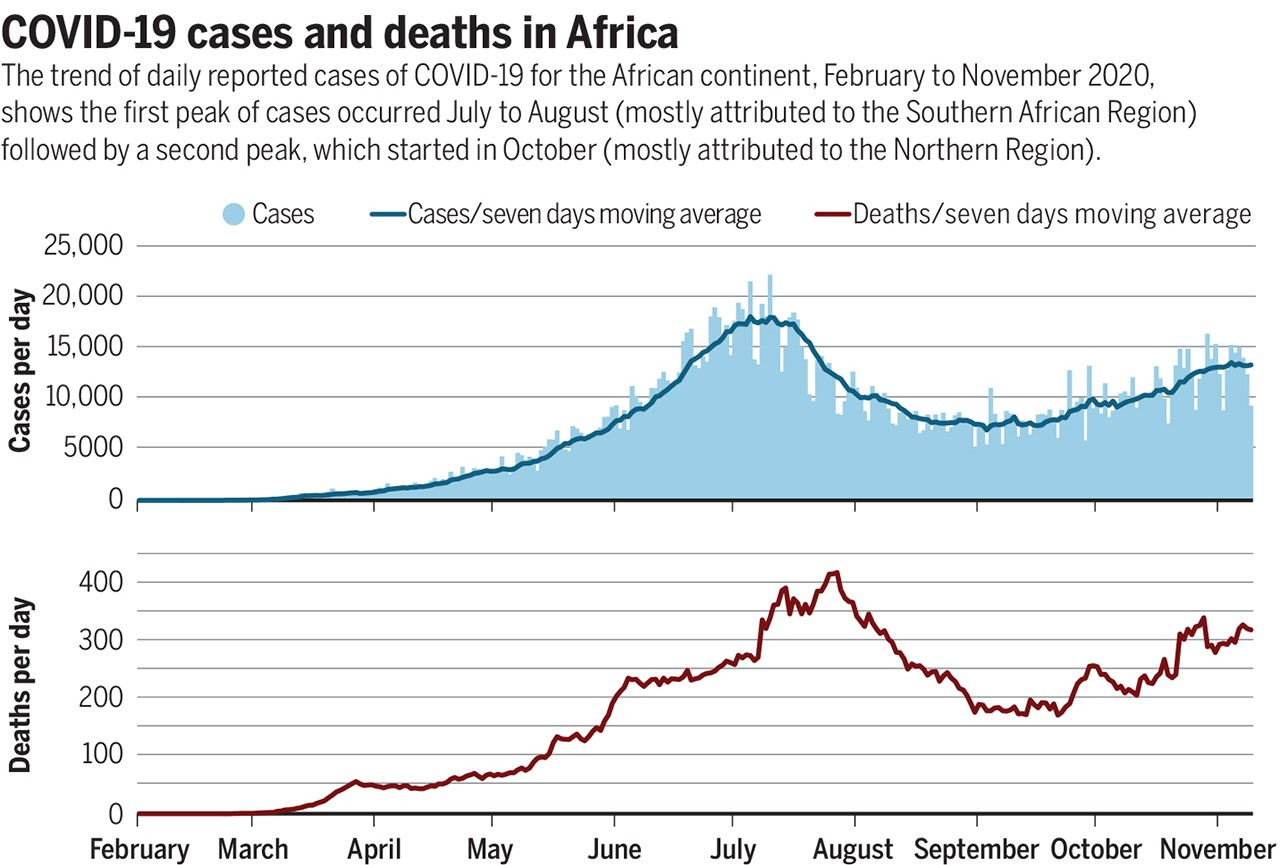
\includegraphics[width=\textwidth]{FIGS/371_27_f1.jpeg}
% "https://doi.org/10.1126/science.abf8832")
\end{frame}


\begin{frame}{Some terminology for ``where''}
- \defword{Epidemic}: diseases that are *visited upon* a population
\vfill
- \defword{Pandemic}: (will revisit this later in the course) epidemic that has spread across a large region, e.g., multiple continents or worldwide
\vfill
- \defword{Endemic}: diseases that *reside within* a population
\vfill
- We don't say "panendemic"
\end{frame}


\begin{frame}{Where? \href{https://en.wikipedia.org/wiki/1854_Broad_Street_cholera_outbreak}{1854 cholera outbreak}}
    \begin{minipage}{0.5\textwidth}
    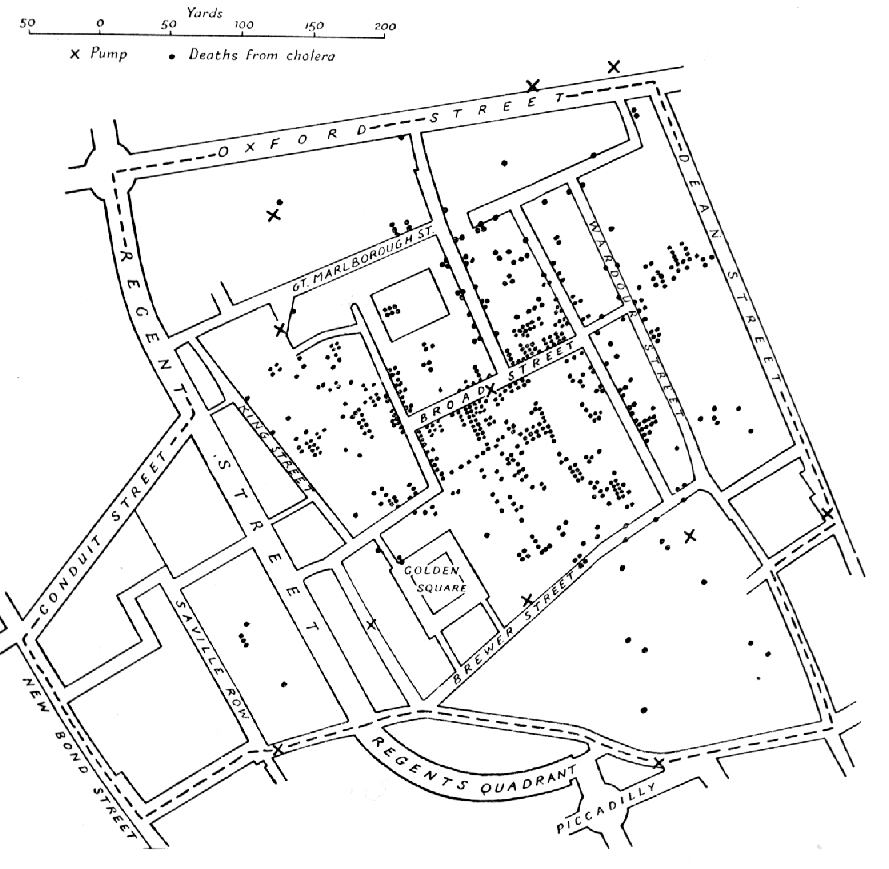
\includegraphics[width=\textwidth]{FIGS/Snow-cholera-map.jpg}
    \end{minipage}
    \begin{minipage}{0.45\textwidth}
        Cholera outbreak near Broad Street, London (UK)
        \vfill
        Studied by \href{https://en.wikipedia.org/wiki/John_Snow}{John Snow}

        \begin{quotation}
            I found that nearly all the deaths had taken place within a short distance of the [Broad Street] pump    
        \end{quotation}
            \end{minipage}
\end{frame}


\begin{frame}{\href{https://www.ncbi.nlm.nih.gov/books/NBK143061/}{WHO pandemic (influenza) phases}}
% <style>
%     .heatMap {
%         overflow:scroll;
%     }
%     .heatMap th {
%         background: grey;
%     }
%     .heatMap tr:nth-child(1) { background: green;}
%     .heatMap tr:nth-child(2) { background: green;}
%     .heatMap tr:nth-child(3) { background: yellow;}
%     .heatMap tr:nth-child(4) { background: yellow;}
%     .heatMap tr:nth-child(5) { background: orange;}
%     .heatMap tr:nth-child(6) { background: red;}
% </style>

% <div class="heatMap">

\begin{tabular}{ccp{6cm}}
Period & Phase & Description \\
\hline
\rowcolor{lgreen} \color{black}Interpandemic & \color{black}1 & \color{black} No animal influenza virus circulating among animals has been reported to cause infection in humans \\
\rowcolor{lgreen} & \color{black}2 & \color{black}Animal influenza virus circulating in domesticated or wild animals known to have caused infection in humans and therefore considered a specific potential pandemic threat
\end{tabular}
\end{frame}

\begin{frame}{\href{https://www.ncbi.nlm.nih.gov/books/NBK143061/}{WHO pandemic (influenza) phases}}
\begin{tabular}{ccp{6cm}}
Period & Phase & Description \\
\hline 
\rowcolor{yellow} \color{black}Pandemic alert & \color{black}3 & \color{black}Animal or human-animal influenza reassortant virus has caused sporadic cases or small clusters of disease in people, but has not resulted in H2H transmission sufficient to sustain community-level outbreaks \\
\rowcolor{yellow} & \color{black}4 & \color{black}Human-to-human transmission of an animal or human-animal influenza reassortant virus able to sustain community-level outbreaks has been verified 
\end{tabular}
\end{frame}

\begin{frame}{\href{https://www.ncbi.nlm.nih.gov/books/NBK143061/}{WHO pandemic (influenza) phases}}
\begin{tabular}{ccp{6cm}}
    Period & Phase & Description \\
    \hline 
\rowcolor{orange} \color{black}Pandemic alert & \color{black} 5 & \color{black} Same identified virus has caused sustained community-level outbreaks in at least 2 countries in 1 WHO region \\
\rowcolor{lred} \color{black}Pandemic & \color{black}6 & \color{black}In addition to criteria in Phase 5, same virus has caused sustained community-level outbreaks in at least 1 other country in another WHO region
\end{tabular}
\end{frame}

\begin{frame}
    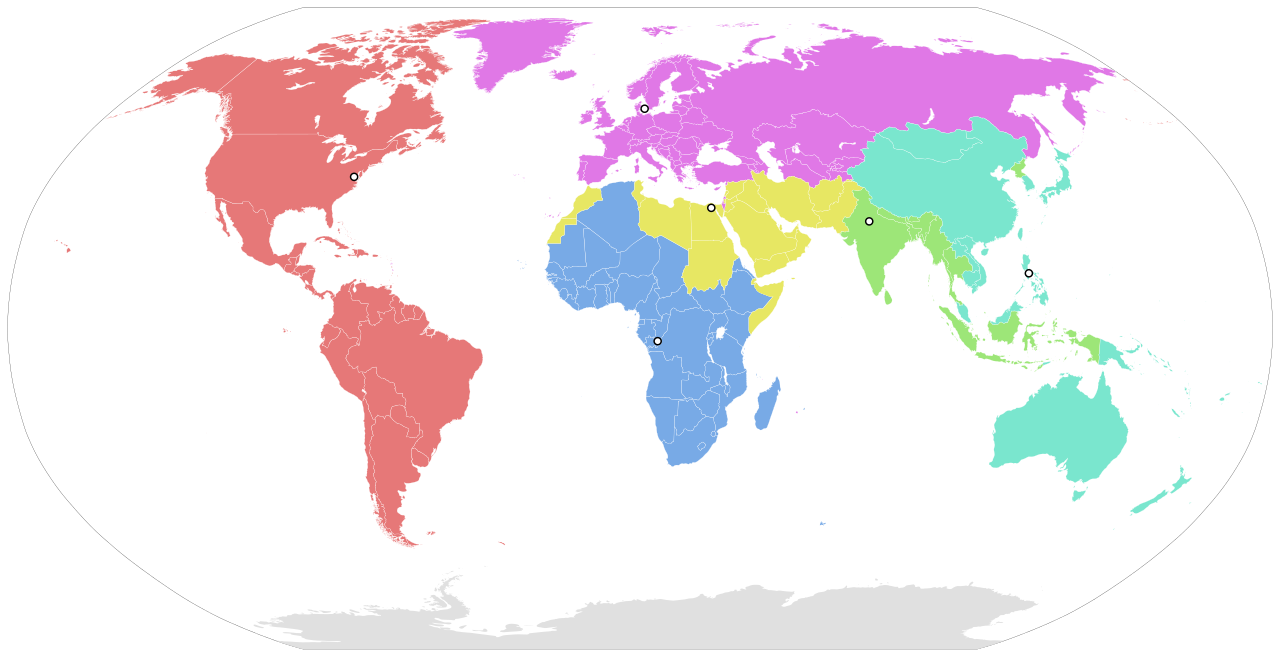
\includegraphics[width=\textwidth]{FIGS/1280px-World_Health_Organisation_regional_offices.png}
\end{frame}



%%%%%%%%%%%%%%%%%%%%
%%%%%%%%%%%%%%%%%%%%
\subsection{Fighting against infections}

\begin{frame}{Fighting against infections}
\begin{quote}
    Epidemiological information is used to plan and evaluate \defword{strategies to prevent illness} and as a guide to the \defword{management of patients} in whom disease has already developed  
\end{quote}
\vfill
- Preventing illness
\begin{itemize}
    \item Prophylactic measures
    \item Vaccination
\end{itemize}
\vfill
- Managing illness
\begin{itemize}
    \item Prevention of further spread (e.g., in hospital) 
    \item Treatment
\end{itemize}
\end{frame}


\begin{frame}{Immunisation}
- Smallpox first disease for which it was known 
\vfill
- Mentioned in a 1549 Chinese book
\vfill
- China: powdered smallpox scabs blown up noses of the healthy; variolation-induced mortality not negligible (0.5-2\%) but lower than normal (20\%)
\vfill
- 1798:  Edward Jenner introduces safer inoculation with cowpox (vaccination)
\vfill
- 1880s: Pasteur extends vaccination to chicken cholera and anthrax in animals and human rabies
\vfill
At the time, *herd immunity* was not understood so this was for personal protection
\end{frame}


\begin{frame}
<div style = "position: relative; top: -55%; padding-bottom:60px; font-size:40px">
Measles cases in the USA
</div>
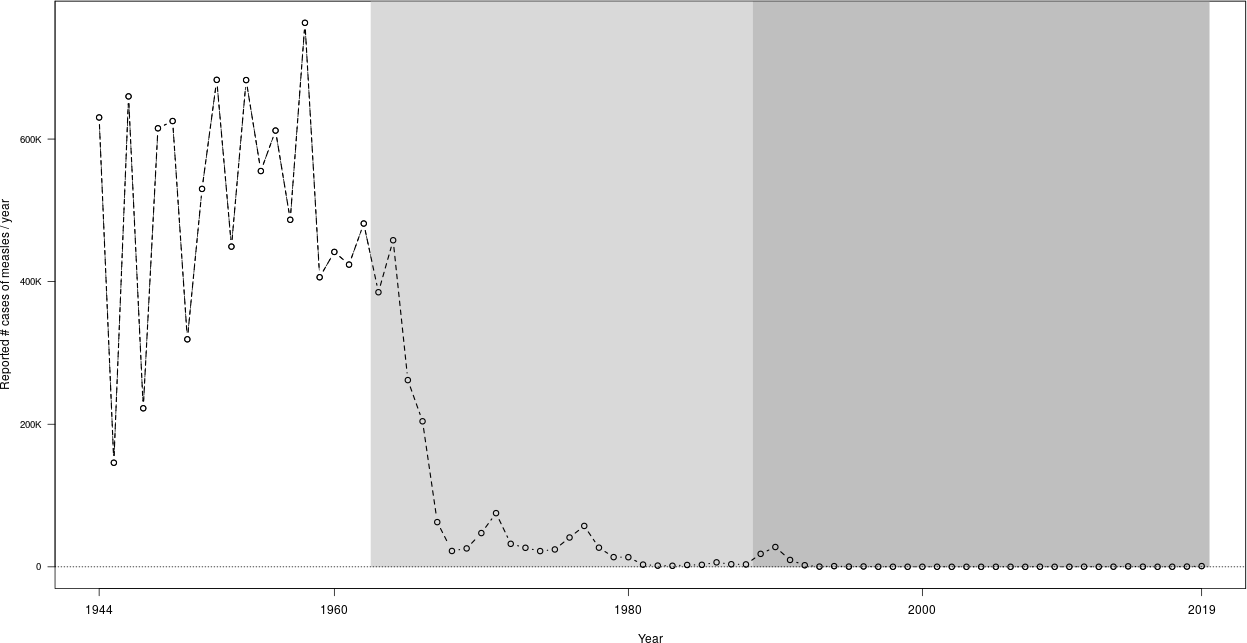
\includegraphics[width=\textwidth]{FIGS/measles_US_1944_2019.png}
\end{frame}


%%%%%%%%%%%%%%%%%%%%
%%%%%%%%%%%%%%%%%%%%
%%%%%%%%%%%%%%%%%%%%
%%%%%%%%%%%%%%%%%%%%
\section{Mathematical Epidemiology}

\begin{frame}{The domain is quite old ..}
.. but has only become a thing in recent years!
\end{frame}

%%%%%%%%%%%%%%%%%%%%
%%%%%%%%%%%%%%%%%%%%
\subsection{The early years}
\begin{frame}{Daniel Bernoulli (1760)}
\begin{minipage}{0.5\textwidth}
    
\includegraphics[width=\textwidth]{FIGS/Bernoulli-1760-first_page.jpg}
\end{minipage}
\begin{minipage}{0.47\textwidth}
- \href{https://gallica.bnf.fr/ark:/12148/bpt6k3558n/f220.item}{BNF scan} or \href{https://julien-arino.github.io/assets/pdf/Bernoulli-1760.pdf}{pdf}
\vfill
- Probably the first epidemic model
\vfill
- About petite vérole (smallpox) inoculation    
\end{minipage}
\end{frame}


\begin{frame}{Ross (early 1900)}
\begin{minipage}{0.5\textwidth}
    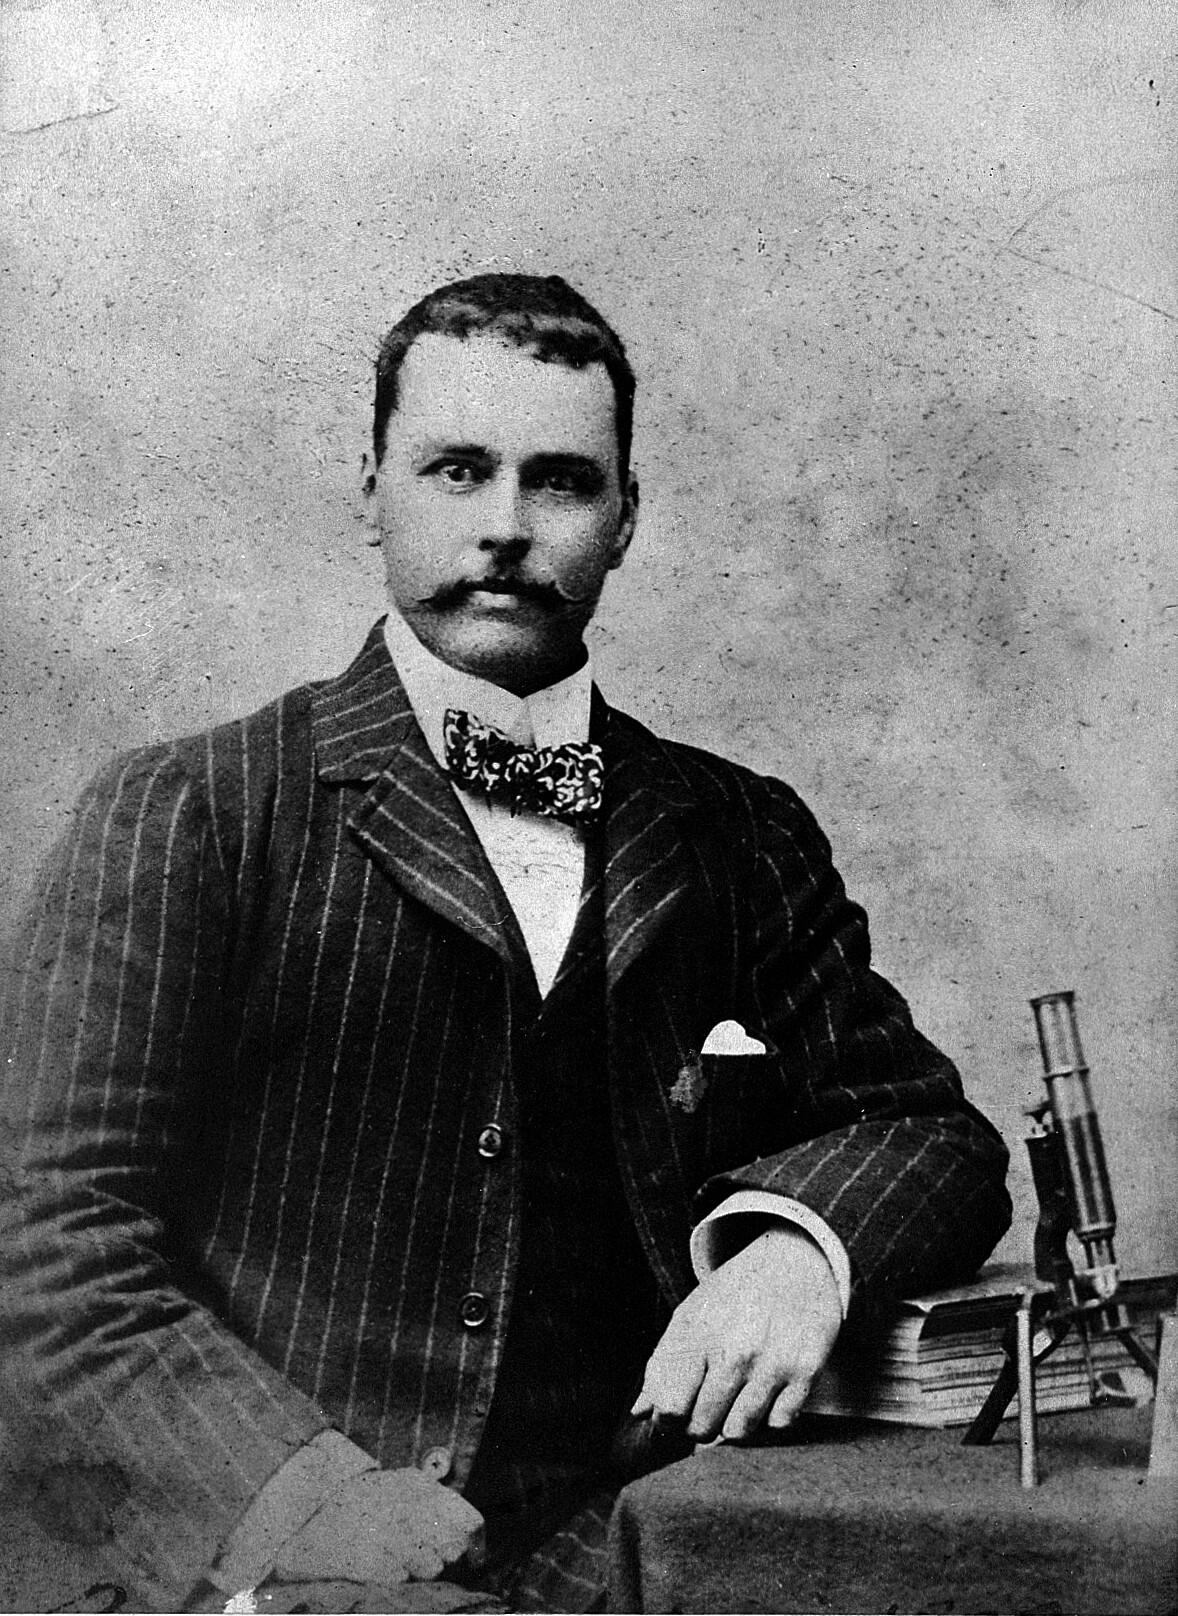
\includegraphics[width=\textwidth]{FIGS/RonaldRoss_WellcomeCollection.jpg}
\end{minipage}
\begin{minipage}{0.47\textwidth}
- On 20 August 1897, observed malaria parasites in the gut of a mosquito fed several days earlier on a malaria positive human
\vfill
- Nobel Prize for Medicine 1902
\vfill
- Started considering malaria eradication using mathematical models; for some history, read \href{https://www.ncbi.nlm.nih.gov/pmc/articles/PMC3320609/pdf/ppat.1002588.pdf}{this 2012 paper}
\end{minipage}
\end{frame}


\begin{frame}{Kermack and McKendrick (1927+)}

- We spend a lot more time on this later
\vfill
- Groundbreaking set of papers starting in 1927
\vfill
- We will see one particular case, the most well known, but this is just the tip of the iceberg of their work
\end{frame}

\begin{frame}{Macdonald, Dietz and malaria}
- Read for instance \href{https://doi.org/10.1371/journal.ppat.1002588}{this paper}, which presents a history of the development of the so-called Ross-Macdonald model
\vfill
- Klaus Dietz also worked a lot on malaria
\end{frame}
    
    
\begin{frame}{Some activity later, but not much until 1990s}
- In recent years, explosion
\vfill
- Since the beginning of COVID-19: just nuts..
\end{frame}

\begin{frame}{Some landmarks in mathematical epidemiology (IMBO)}
- Macdonald. The epidemiology and control of malaria. 1957
\vfill
- Baroyan, Rvachev et al. Deterministic epidemic models for a territory with a transport network. Kibernetika, 1967
\vfill
- Hethcote \& Yorke. Gonorrhea Transmission Dynamics and Control. LNBM 56, 1984
\vfill
- Anderson \& May. Infectious diseases of humans: dynamics and control. 1991
\vfill
- Capasso. Mathematical Structures of Epidemic Systems. LNBM 97, 1993
\vfill
- Hethcote. The mathematics of infectious diseases. SIAM Review, 2000
\vfill
- van den Driessche \& Watmough. Reproduction numbers and sub-threshold endemic equilibria for compartmental models of disease transmission. MBS, 2002      
\end{frame}


%%%%%%%%%%%%%%%%%%%%
%%%%%%%%%%%%%%%%%%%%
\subsection{Computational epidemiology}

\begin{frame}{A more recent trend}
- Some rare numerical work $\leq$ 1980s, mostly simulation of math models
\begin{itemize}
    \item Baroyan, Rvachev et al. \href{https://doi.org/10.2307/1426167}{Computer modelling of influenza epidemics for the whole country (USSR)}. \emph{Advances in Applied Probability} (1971) 
    \item Rvachev \& Longini. \href{https://doi.org/10.1016/0025-5564(85)90064-1}{A mathematical model for the global spread of influenza}. \emph{Mathematical Biosciences} (1986) 
    \item Flahault, Letrait et al. \href{https://doi.org/10.1002/sim.4780071107}{Modelling the 1985 influenza epidemic in France}. \emph{Statistics in Medicine} (1988)
\end{itemize}
\vfill
- More and more frequent now, to the point that some modelling studies are purely simulation-based
\end{frame}

\begin{frame}{Agent-based models (ABM)}
- Early in the life of these models, they were called IBM (individual-based models)
\vfill
- Over the years, a "philosophical" distinction has emerged:
    - IBM are mathematical models that consider individuals as the units; e.g., DTMC, CTMC, branching processes, etc.
    - ABM are computational models whose study is, for the most part, only possible numerically 
\end{frame}

\begin{frame}{Network models}
- Network models endow vertices with simple systems and couple them through graphs
\vfill
- Can be ABM, but some networks can also be studied analytically

\end{frame}

%%%%%%%%%%%%%%%%%%%%
%%%%%%%%%%%%%%%%%%%%
\subsection{Use of data in epidemiology}

\begin{frame}{Has happened all along, undergoing a transformation}
- Epidemiology has long relied on data
\vfill
- Many developments in statistics originate there
\vfill
- Data has traditionally been better for chronic diseases than for infectious ones
\vfill
- Near-real-time surveillance of infectious diseases ongoing since the 1980s (e.g., Réseau Sentinelles)
\vfill
- SARS-CoV-1 saw the beginning of a move towards real-time emerging infectious disease data
\vfill
- With SARS-CoV-2, the system has really progressed a lot, both in terms of "citizen science" and governmental initiatives
\end{frame}



%%%%%%%%%%%%%%%%%%%%
%%%%%%%%%%%%%%%%%%%%
%%%%%%%%%%%%%%%%%%%%
%%%%%%%%%%%%%%%%%%%%
\section{Compartmental models}

\begin{frame}{Compartmental models}
- Have become synonymous with epidemiological models
\vfill
- Many epidemiological models are compartmental models, but the development of compartmental models in the 1970-1980s was not at all specific to epidemiology
\vfill
- See in particular the works of John Jacquez, Carl Simon, GG Walter
\vfill
- Unjustly fell into disuse: there are some very nice results in the area    
\end{frame}

\begin{frame}{Compartment (\href{https://doi-org.uml.idm.oclc.org/10.1016/B978-0-12-434180-7.50021-8}{Jacquez 1979})}

\begin{quote}
  A \defword{compartment} is an amount of some material which acts kinetically like a distinct, homogeneous, well-mixed amount of material. A \defword{compartmental system} consists of one or more compartments which interact by exchanging the material. There may be inputs into one or more compartments from outside the system and there may be excretions from the compartments of the system.   
\end{quote}
\end{frame}

\begin{frame}{}
  \begin{minipage}{0.4\textwidth}
    \tikzstyle{cloud} = [rectangle, 
    draw=yellow!90, 
    fill=yellow!30, 
    thick, 
    minimum width=0.6cm,
    minimum height = 1cm]
    \tikzstyle{line} = [draw, 
    -latex', 
    color=black]
    \begin{tikzpicture}[scale=1.5, transform shape]
      \node [cloud] (S) {$q_i$};
      \coordinate[above=of S] (h1);
      \coordinate[right=of S] (h2);
      \coordinate[left=of S] (h3);
      \coordinate[below=of S] (h4);
      %% Flows
      \path [line, very thick] (h1) to node [midway, right] (TextNode) {$i_i(t)$} (S);
      \path [line, very thick] (S) to node [midway, above] (TextNode) {$f_{ji}$} (h2);
      \path [line, very thick] (h3) to node [midway, above] (TextNode) {$f_{ij}$} (S);
      \path [line, very thick] (S) to node [midway, right] (TextNode) {$f_{0i}$} (h4);
    \end{tikzpicture}  
  \end{minipage}
  \begin{minipage}{0.55\textwidth}
    \begin{itemize}
      \item $q_i$ size of the compartment, i.e., quantity of kinetically homogeneous material present in $i$; $q_i\geq 0$ 
      \item $f_{ij}$ and $f_{ji}$ transfer coefficients/functions
      \item $f_{0i}$ excretion coefficient/function
      \item $i_i(t)$ entries from outside the system
    \end{itemize}
  \end{minipage}
  \vfill
  Above is a \defword{flow diagram}, which summarises the different flows acting on the compartment
\end{frame}


%%%%%%%%%%%%%%%%%%%%
%%%%%%%%%%%%%%%%%%%%
%%%%%%%%%%%%%%%%%%%%
%%%%%%%%%%%%%%%%%%%%
\section{The Kermack-McKendrick SIR model without demography}

\begin{frame}{Paper series worth reading}
Model here is a particular case in
\begin{itemize}
  \item Kermack \& McKendrick. \href{https://doi.org/10.1098/rspa.1927.0118}{A contribution to the mathematical theory of epidemics} (1927)
\end{itemize}
\vfill
That paper was followed by a series of ``Contributions to the mathematical theory of epidemics.''
\begin{itemize}
  \item \href{https://doi.org/10.1098/rspa.1932.0171}{II. The problem of endemicity} (1932)
  \item \href{https://doi.org/10.1098/rspa.1933.0106}{III. Further studies of the problem of endemicity} (1933)
  \item \href{https://doi.org/10.1017/S0022172400034902}{IV. Analysis of experimental epidemics of the virus disease mouse ectromelia} (1937)
  \item \href{https://doi.org/10.1017/S0022172400011918}{V. Analysis of experimental epidemics of mouse-typhoid; a bacterial disease conferring incomplete immunity} (1939)
\end{itemize}
\end{frame}

\begin{frame}{What is the \emph{size} of an epidemic?}
\bbullet 
If we are interested in the possibility that an epidemic occurs
\begin{itemize}
  \item Does an epidemic peak always take place?
  \item If it does take place, what is its size?
\end{itemize}
\vfill
\bbullet If an epidemic traverses a population, is everyone affected/infected?
\end{frame}


%%%%%%%%%%%%%%%%%%%%
%%%%%%%%%%%%%%%%%%%%
\subsection{The model}
\begin{frame}{The Kermack-McKendrick SIR model without demography}
\bbullet The period of time under consideration is sufficiently short that demography can be neglected (we also say the model has \emph{no vital dynamics})
\vfill
\bbullet Individuals are either \emph{susceptible} to the disease or \emph{infected} by (and \emph{infectious} with) the disease
\vfill
\bbullet After recovering or dying from the disease, individuals are \emph{removed} from the infectious compartment ($R$)
\vfill
\bbullet Incidence is of \defword{mass action} type and takes the form $\beta SI$
\end{frame}


\begin{frame}{Important -- Incidence functions}
Incidence is the rate at which new cases arise, the incidence function then describes how contacts lead to new infections
\vfill
If there are $S$ susceptible individuals and $I$ infectious individuals in the population, we use a function of the form
\[
f(S,I)
\]
The function can also explicitly depend on the total population $N$, i.e., $f(S,I,N)$
\vfill
We return to incidence functions in \href{no.se}{Lecture XY}
\vfill
For now, just know the most common incidence functions are
\begin{itemize}
\item \defword{mass action incidence} $f(S,I,N)=\beta SI$
\item \defword{standard} (or \defword{proportional}) \defword{incidence} $f(S,I,N)=\beta SI/N$
\end{itemize}
\end{frame}


\begin{frame}{The Kermack-McKendrick model}
This model is typically called the Kermack-McKendrick (KMK) SIR model 
\begin{subequations}\label{sys:KMK}
  \begin{align}
    S' &= -\beta SI \tag{1a}\label{sys:KMK_dS} \\
    I' &= \beta SI-\gamma I  \tag{1b}\label{sys:KMK_dI} \\
    R' &= \gamma I  \tag{1c}\label{sys:KMK_dR}
    \end{align}  
\end{subequations}
\vfill
\begin{center}
  \begin{tikzpicture}[scale=1.5, transform shape]
    \node [circle, fill=green!50, text=black] (S) {$S$};
    \node [circle, right=1cm of S, fill=red!90, text=black] (I) {$I$};
    \node [circle, right=1cm of I, fill=blue!90, text=black] (R) {$R$};
    %% Flows
    \path [line, very thick] (S) to node [midway, above] (TextNode) {$\beta SI$} (I);
    \path [line, very thick] (I) to node [midway, above] (TextNode) {$\gamma I$} (R);
  \end{tikzpicture}    
\end{center}
\end{frame}

%%%%%%%%%%%%%%%%%%%%
%%%%%%%%%%%%%%%%%%%%
\subsection{Mathematical analysis}

\begin{frame}{Reduction of the model}
  3 compartments, but when considered in detail, we notice that \emph{removed} do not have a direct influence on the dynamics of $S$ or $I$, in the sense that $R$ does not appear in \eqref{sys:KMK_dS} or \eqref{sys:KMK_dI}
  \vfill
  Furthermore, the total population (including deceased who are also in $R$) $N=S+I+R$ satisfies
  \[
  N'=(S+I+R)'=0
  \]
  Thus, $N$ is constant and the dynamics of $R$ can be deduced from $R=N-(S+I)$
  \vfill
  So we now consider
  \begin{subequations}\label{sys:KMK_2d}
    \begin{align}
      S' &= -\beta SI \label{sys:KMK_2d_dS}\\
      I' &= \beta SI-\gamma I  \label{sys:KMK_2d_dI}
      \end{align}
    \end{subequations}
\end{frame}

\begin{frame}{Equilibria}
  Let us consider the equilibria of
  \begin{subequations}
    \begin{align}
      S' &= -\beta SI 
      \tag{\ref{sys:KMK_2d_dS}} \\
      I' &= (\beta S-\gamma)I  
      \tag{\ref{sys:KMK_2d_dI}}
    \end{align}
  \end{subequations}
\vfill
  From \eqref{sys:KMK_2d_dI}
  \begin{itemize}
    \item either $\bar S=\gamma/\beta$ 
    \item or $\bar I=0$
  \end{itemize}
  \vfill
  Substitute into \eqref{sys:KMK_2d_dS}
  \begin{itemize}
    \item in the first case, $(\bar S,\bar I)=(\gamma/\beta,0)$ 
    \item in the second case, any $\bar S\geq 0$ is an EP
  \end{itemize}
  \vfill
  The second case is an \emph{issue}: the usual linearisation does not work when there is a \emph{continuum} of equilibria as the EP are not \emph{isolated}
\end{frame}


\begin{frame}{Another approach -- Study $dI/dS$}
  \begin{align}
  S' &= -\beta SI \tag{\ref{sys:KMK_2d_dS}}\\
  I' &= \beta SI-\gamma I  \tag{\ref{sys:KMK_2d_dI}}
  \end{align}
  \vfill
  What is the dynamics of $dI/dS$? 
  \begin{equation}
    \label{eq:KMK_dI_over_dS}
    \frac{dI}{dS}
    =\frac{dI}{dt}\frac{dt}{dS}
    =\frac{I'}{S'}
    =\frac{\beta SI-\gamma I}{-\beta SI}
    =\frac{\gamma}{\beta S}-1
  \end{equation}
 provided $S\neq 0$
  \vfill
  \textbf{Note --} Recall that $S$ and $I$ are $S(t)$ and $I(t)$.. \eqref{eq:KMK_dI_over_dS} thus describes the relation between $S$ and $I$ over solutions to the original ODE \eqref{sys:KMK_2d}
\end{frame}


\begin{frame}{}
  Integrate $\eqref{eq:KMK_dI_over_dS}$ and obtain trajectories in state space
  $$
  I(S)=\frac\gamma\beta \ln S-S+C
  $$
  with $C\in\mathbb{R}$
  \vfill
  IC $I(S_0)=I_0$ $\Rightarrow$ $C=S_0+I_0-\dfrac \gamma\beta \ln S_0$ and the solution to \eqref{sys:KMK} is, as a function of $S$
  \begin{align*}
  I(S)&=S_0+I_0-S+\frac\gamma\beta \ln \frac S{S_0} \\
  R(S)&=N-S-I(S)=R_0-\frac\gamma\beta \ln \frac S{S_0}
  \end{align*}
  (since $N_0=S_0+I_0+R_0$)
\end{frame}


\begin{frame}{}
  Trajectories of \eqref{sys:KMK_2d} in $(S,I)$-space, normalised, with IC $(S_0,1-S_0)$ and $\beta/\gamma=2.5$
  \vfill
\begin{center}
  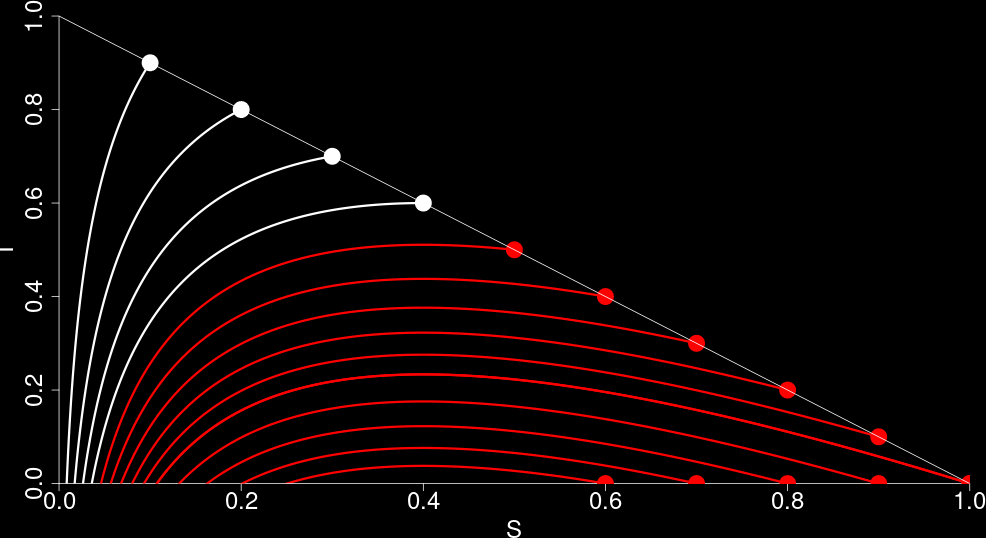
\includegraphics[width=\textwidth]{FIGS/KMK_planar_trajectories.png}
\end{center}
\end{frame}


\begin{frame}{}
  Let us study
  $$
  I(S)=S_0+I_0-S+\frac\gamma\beta \ln \frac S{S_0} 
  $$
  We have
  $$
  \frac{d}{dS}I(S) = \frac{\gamma}{\beta S}-1
  $$
  So, in the previous curves, the max of $I(S)$ happens when $S=\gamma/\beta$ ($S=0.4$ in the example)
  \vfill
  At that point,
  $$
  I(S) = I_0+\left(
    1-\frac{1}{\R_0} - \frac{\ln(\R_0)}{\R_0}
  \right)S_0
  $$
\end{frame}


\begin{frame}{}
  \begin{theorem}[Epidemic or no epidemic?]
    Let $(S(t),I(t))$ be a solution to \eqref{sys:KMK_2d} and $\R_0$ defined by
    \begin{equation}\label{eq:R0_KMK}
    \R_0=\frac{\beta}{\gamma}S_0
    \end{equation}
    \vfill
    \begin{itemize}
      \item If $\R_0\leq 1$, then $I(t)\searrow 0$ when $t\to\infty$ 
      \item If $\R_0>1$, then $I(t)$ first reaches a maximum 
      \begin{equation}\label{eq:max_I}
        I_0+\left(
      1-\frac{1}{\R_0} - \frac{\ln(\R_0)}{\R_0}
      \right)S_0
      \end{equation}
      then goes to 0 as $t\to\infty$  
    \end{itemize}    
  \end{theorem}
\end{frame}


\begin{frame}[fragile]{}
\begin{lstlisting}
rhs_SIR_KMK <- function(t, x, p) {
  with(as.list(c(x, p)), {
    dS = - beta * S * I
    dI = beta * S * I - gamma * I
    dR = gamma * I
    return(list(c(dS, dI, dR)))
  })
}
# Initial condition for S (to compute R_0)
S0 = 1000
gamma = 1/14
# Set beta so that R_0 = 1.5
beta = 1.5 * gamma / S0 
params = list(gamma = gamma, beta = beta)
IC = c(S = S0, I = 1, R = 0)
times = seq(0, 365, 1)
sol <- ode(IC, times, rhs_SIR_KMK, params)  
\end{lstlisting}
\end{frame}


\begin{frame}[fragile]{}
\begin{lstlisting}
plot(sol[, "time"], sol[, "I"], type = "l",
main = TeX("Kermack-McKendrick SIR, $R_0=1.5$"),
xlab = "Time (days)", ylab = "Prevalence")
\end{lstlisting}
\begin{center}
\includegraphics[width=\textwidth]{FIGS/lecture-01-introduction-math-epi-KMK_R0eq1dot5}
\end{center}
\end{frame}


\begin{frame}{The basic reproduction number $\R_0$}
\bbullet Indicator often used in epidemiology. Verbally
\begin{quote}
  average number of secondary cases of infection produced when a single infectious individual is introduced in a wholly susceptible population
\end{quote}
\vfill
\bbullet If $\R_0<1$, then each infectious individual infects on average less than 1 person and the epidemic is quite likely to go extinct 
\vfill
\bbullet If $R_0>1$, then each infectious individual infects on average more than 1 person and an epidemic is quite likely to occur
\end{frame}

\begin{frame}{A few sample values of $\R_0$}
  $\R_0$ can be estimated from data
  \vfill
  \begin{center}
  \begin{tabular}{llcc}
  \hline 
  Infection & Location & Period & $\R_0$ \\
  \hline
  Measles & Cirencester, England & 1947-50 & 13-14 \\
  & England and Wales & 1950-68 & 16-18 \\
  & Kansas, USA & 1918-21 & 5-6 \\
  & Ontario, Canada & 1912-3 & 11-12 \\
  & Willesden, England & 1912-3 & 11-12 \\
  & Ghana & 1960-8 & 14-15 \\
  & East Nigeria & 1960-8 & 16-17 \\
  \end{tabular}
  \end{center}
\end{frame}
    

%%%%%%%%%%%%%%%%%%%%%%%%
%%%%%%%%%%%%%%%%%%%%%%%%
\subsection{The final size of an epidemic}

\begin{frame}{Final size of an epidemic}
  For a nonnegative valued integrable function $w(t)$, denote
  $$
  w_\infty = \lim_{t\to\infty}w(t),\qquad\hat w = \int_0^\infty w(t)\ dt
  $$
  Denote $w_0=w(0)$. In the subsystem
  \begin{align}
  S' &= -\beta SI \tag{\ref{sys:KMK_2d_dS}} \\
  I' &= \beta SI-\gamma I \tag{\ref{sys:KMK_2d_dI}} 
  \end{align}
  compute the sum of \eqref{sys:KMK_2d_dS} and \eqref{sys:KMK_2d_dI}, making sure to show time dependence $$
  \frac{d}{dt}(S(t)+I(t))=-\gamma I(t)
  $$
\end{frame}


\begin{frame}{}
  Integrate from 0 to $\infty$:
  $$
  \int_0^\infty\frac{d}{dt}(S(t)+I(t))\ dt=-\int_0^\infty\gamma I(t)dt 
  $$
  The left hand side gives
  $$
  \int_0^\infty\frac{d}{dt}(S(t)+I(t))\ dt
  = S_\infty+I_\infty-S_0-I_0 = S_\infty-S_0-I_0
  $$
  since $I_\infty=0$
  \vfill
  The right hand side takes the form
  $$
  -\int_0^\infty\gamma I(t)dt = -\gamma\int_0^\infty I(t)dt = -\gamma \hat I
  $$
  We thus have
  \begin{equation}
  \label{eq:KMK_final_size_step1}
  S_\infty-S_0-I_0 = -\gamma\hat I
  \end{equation}
\end{frame}



\begin{frame}{}
  Now consider \eqref{sys:KMK_2d_dS}:
  $$
  S' = -\beta SI
  $$
  Divide both sides by $S$:
  $$
  \frac{S'(t)}{S(t)} = -\beta I(t)
  $$
  Integrate from 0 to $\infty$:
  \begin{equation}
  \label{eq:KMK_final_size_step2}
  \ln S_\infty-\ln S_0 = -\beta \hat I
  \end{equation}
  Express \eqref{eq:KMK_final_size_step1} and \eqref{eq:KMK_final_size_step2} in terms of $-\hat I$ and equate
  $$
  \frac{\ln S_\infty-\ln S_0}{\beta}
  =
  \frac{S_\infty-S_0-I_0}{\gamma}
  $$
  Thus we have
  \begin{equation}
  \label{eq:final_size}
  (\ln S_0-\ln S_\infty)S_0 = (S_0-S_\infty)\R_0+I_0\R_0
  \end{equation}
\end{frame}



\begin{frame}{}
\begin{theorem}[Final size relation]
  Let $(S(t),I(t))$ be a solution to \eqref{sys:KMK_2d} and $\R_0$ defined by \eqref{eq:R0_KMK}
  \vskip0.5cm
  The number $S(t)$ of susceptible individuals is a nonincreasing function and its limit $S_\infty$ is the only solution in $(0,S_0)$ of the transcendental equation
  \begin{equation}\tag{\ref{eq:final_size}}
  (\ln S_0-\ln S_\infty)S_0 = (S_0-S_\infty)\R_0+I_0\R_0
  \end{equation}
\end{theorem}
\end{frame}



\begin{frame}{The (transcendantal) final size equation}
  Rewrite the final size equation
  \begin{equation}
    \tag{\ref{eq:final_size}}
  (\ln S_0-\ln S_\infty)S_0 = (S_0-S_\infty)\R_0+I_0\R_0
  \end{equation}
  as
  \begin{equation}
  \label{eq:final_size_2}
  T(S_\infty) =(\ln S_0-\ln S_\infty)S_0
  - (S_0-S_\infty)\R_0 -I_0\R_0
\end{equation}
\vfill
Thus, we seek the zeros of the function $T(S_\infty)$
\end{frame}



\begin{frame}{}
  We seek $S_\infty$ in $(0,S_0]$ s.t. $T(S_\infty)=0$, with
  \begin{equation}\tag{\ref{eq:final_size_2}}
    T(S_\infty) =(\ln S_0-\ln S_\infty)S_0
    - (S_0-S_\infty)\R_0 -I_0\R_0      
  \end{equation}
  \vfill
  Note to begin that 
  $$
  \lim_{S_\infty\to 0}T(S_\infty)=\lim_{S_\infty\to 0}-S_0\ln(S_\infty)=\infty
  $$
  \vfill
  Differentiating $T$ with respect to $S_\infty$, we get 
  $$
  T'(S_\infty)=\R_0-S_0/S_\infty
  $$ 
  \vfill
  When $S_\infty\to 0$, $\R_0-S_0/S_\infty<0$, so $T$ decreases to $S_\infty=S_0/\R_0$
  \vfill
  So if $\R_0\leq 1$, the function $T$ is decreasing on $(0,S_0)$, while it has a minimum if $\R_0>1$
\end{frame}



\begin{frame}{Case $\R_0\leq 1$}
  \begin{equation}\tag{\ref{eq:final_size_2}}
    T(S_\infty) =(\ln S_0-\ln S_\infty)S_0
    - (S_0-S_\infty)\R_0 -I_0\R_0      
  \end{equation}
  \vfill
  \bbullet We have seen that $T$ decreases on $(0,S_0]$
  \vfill
  \bbullet Also, $T(S_0)=-I_0\R_0<0$ ($I_0=0$ is trivial and not considered)
  \vfill
  \bbullet $T$ is continuous
  \vfill
  $\implies$ there exists a unique $S_\infty\in (0,S_0]$ s.t. $T(S_\infty)=0$
\end{frame}


\begin{frame}{Case $\R_0> 1$}
  \begin{equation}\tag{\ref{eq:final_size_2}}
    T(S_\infty) =(\ln S_0-\ln S_\infty)S_0
    - (S_0-S_\infty)\R_0 -I_0\R_0      
  \end{equation}
  \vfill
  \bbullet We have seen that $T$ decreases on $(0,S_0/\R_0]$
  \vfill
  \bbullet For $S_\infty\in[S_0/\R_0]$, $T'>0$
  \vfill
  \bbullet As before, $T(S_\infty)=-I_0\R_0$
  \vfill
  \bbullet $T$ is continuous
  \vfill
  $\implies$ there exists a unique $S_\infty\in (0,S_0]$ s.t. $T(S_\infty)=0$. More precisely, in this case, $S_\infty\in(0,S_0/\R_0)$
\end{frame}



\begin{frame}[fragile]{}
We solve numerically. We need a function
\begin{lstlisting}  
final_size_eq = function(S_inf, S0 = 999, I0 = 1, R_0 = 2.5) {
  OUT = S0*(log(S0)-log(S_inf)) - (S0+I0-S_inf)*R_0
  return(OUT)
}
\end{lstlisting}
and solve easily using \code{uniroot}, here with the values by default that we have set for the function
\begin{lstlisting}
uniroot(f = final_size_eq, interval = c(0.05, 999))
$root
[1] 106.8819
$f.root
[1] -2.649285e-07
$iter
[1] 10
$init.it
[1] NA
$estim.prec
[1] 6.103516e-05
\end{lstlisting}
\end{frame}


\begin{frame}[fragile]{}
To use something else than the default values, e.g.,
\vfill
\begin{lstlisting}  
N0 = 1000
I0 = 1
S0 = N0-I0
R_0 = 2.4
uniroot(
  f = function(x) 
    final_size_eq(S_inf = x, 
                  S0 = S0, I0 = I0, 
                  R_0 = R_0),
  interval = c(0.05, S0))
\end{lstlisting}
\end{frame}


\begin{frame}[fragile]{A figure with all the information}
\begin{lstlisting}
S = seq(0.1, S0, by = 0.1)
fs = final_size(S, S0 = S0, I0 = I0, R_0 = R_0)
S_inf = uniroot(f = function(x) final_size_eq(S_inf = x, 
                                              S0 = S0, I0 = I0, 
                                              R_0 = R_0),
                interval = c(0.05, S0))
plot(S, fs, type = "l", ylab = "Value of equation (10)")
abline(h = 0)
points(x = S_inf$root, y = 0, pch = 19)
text(x = S_inf$root, y = 0, labels = "S_inf", adj = c(-0.25,-1))    
\end{lstlisting}
\end{frame}


\begin{frame}{$\R_0=0.8$}
\begin{center}
  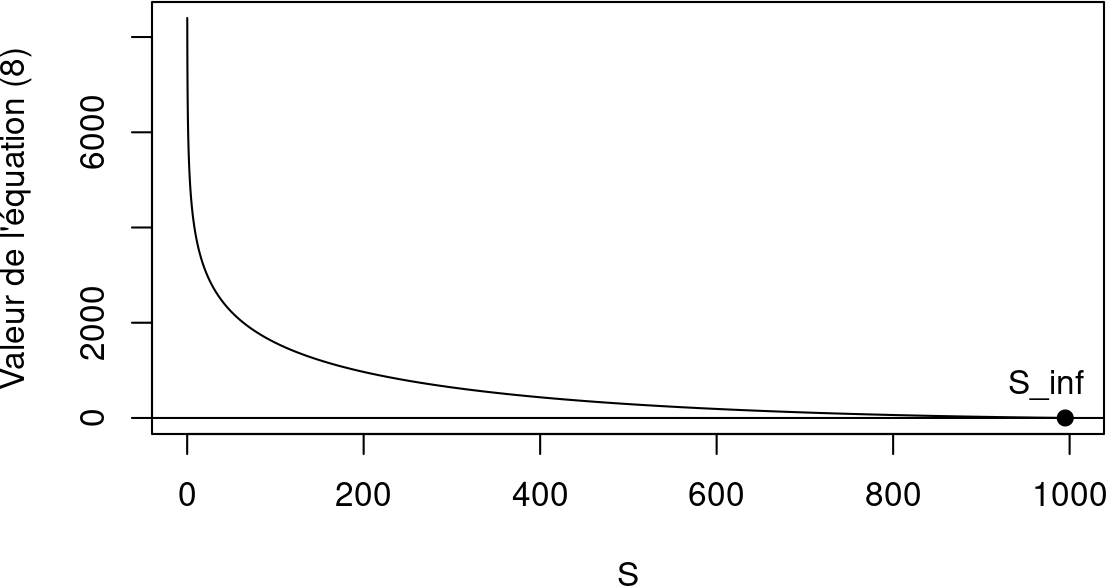
\includegraphics[width=\textwidth]{FIGS/KMK_final_size_R0_0p8}
\end{center}
\end{frame}


\begin{frame}{$\R_0=2.4$}
  \begin{center}
    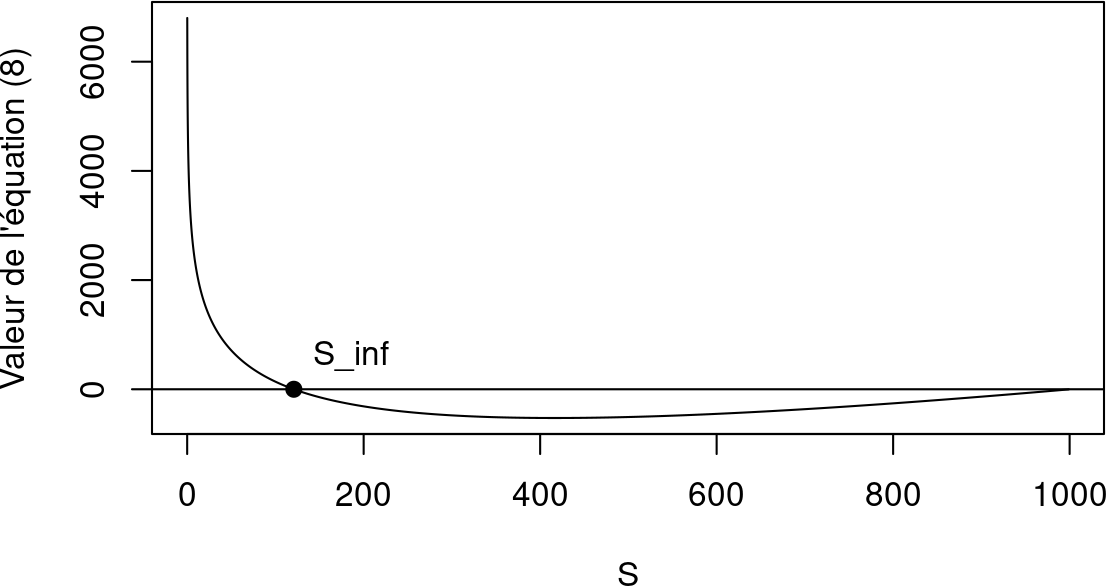
\includegraphics[width=\textwidth]{FIGS/KMK_final_size_R0_2p4}
  \end{center}
\end{frame}


\begin{frame}[fragile]{A little nicer}
\begin{lstlisting}
values = expand.grid(
  R_0 = seq(0.01, 3, by = 0.01),
  I0 = 1:100
)
values$S0 = N0-values$I0
L = split(values, 1:nrow(values))

values$S_inf = sapply(X = L, FUN = final_size)

values$taille_finale = values$S0-values$S_inf+values$I0
values$taux_attaque = (values$taille_finale / N0)*100

levelplot(taux_attaque ~ R_0*I0, data = values, 
          xlab="R_0", ylab = "I0",
          col.regions = viridis(100))  
\end{lstlisting}
(requires \code{lattice} and \code{viridis} librairies)
\end{frame}


\begin{frame}{Attack rate (in \%)}
  \begin{center}
    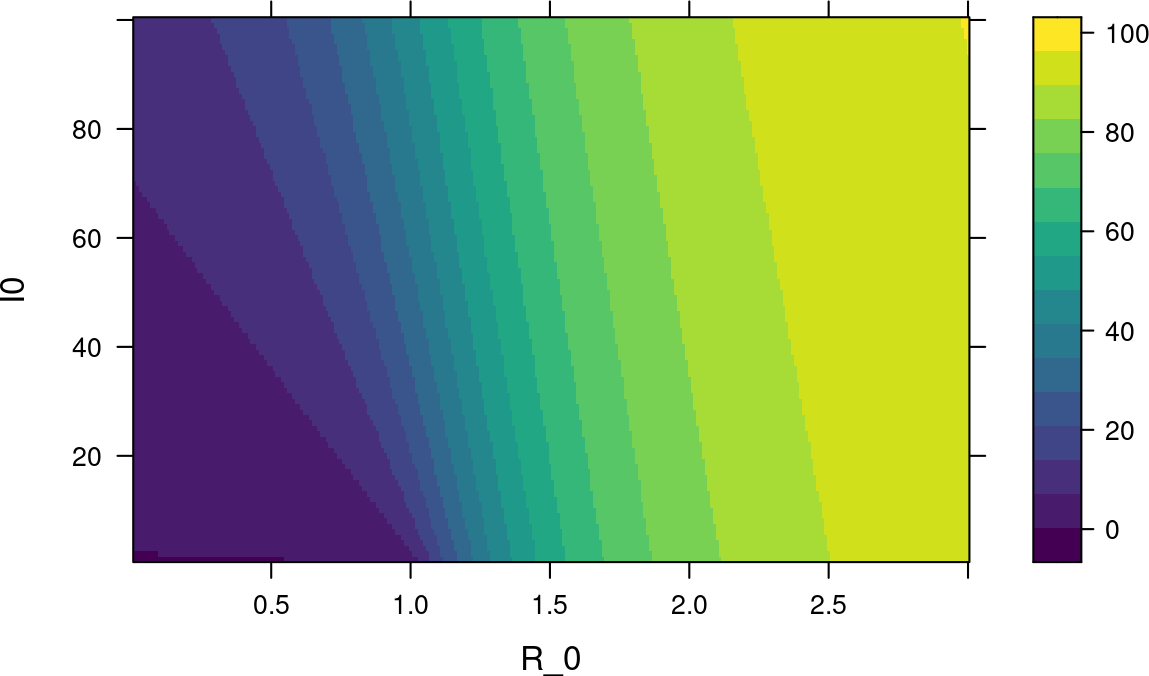
\includegraphics[width=\textwidth]{FIGS/KMK_taux_attaque}
  \end{center}
\end{frame}


%%%%%%%%%%%%%%%%%%%%%%%%%%%
%%%%%%%%%%%%%%%%%%%%%%%%%%%
\subsection{Herd immunity}

\begin{frame}{The simplest vaccination model}
To implement vaccination in KMK, assume that vaccination reduces the number of susceptibles
\vfill
Let total population be $N$ with $S_0$ initially susceptible
\vfill
Vaccinate a fraction $p\in[0,1]$ of susceptible individuals
\vfill
Original IC (for simplicity, $R(0)=0$)
\begin{equation}\label{eq:IC_KMK_novacc}
IC: (S(0),I(0),R(0)) = (S_0,I_0,0)
\end{equation}
Post-vaccination IC 
\begin{equation}\label{eq:IC_KMK_vacc}
IC: (S(0),I(0),R(0)) = ((1-p)S_0,I_0,pS_0)
\end{equation}
\end{frame}


\begin{frame}{Vaccination reproduction number}
  Without vaccination
  \begin{equation}\tag{\ref{eq:R0_KMK}}
    \R_0=\frac{\beta}{\gamma}S_0
  \end{equation}
  \vfill
  With vaccination, denoting $\R_0^{\text{v}}$ the reproduction number,
  \begin{equation}
    \R_0^{\text{v}} = \frac{\beta}{\gamma}(1-p)S_0
  \end{equation}
  \vfill
  Since $p\in[0,1]$, $\R_0^{\text{v}}\leq\R_0$
\end{frame}


\begin{frame}{Herd immunity}
  Therefore
  \begin{itemize}
    \item $\R_0^{\textrm{v}}<\R_0$ if $p>0$ 
    \item To control the disease, $\R_0^{\text{v}}$ must take a value less than 1
  \end{itemize}
  \vfill
To make $\R_0^{\text{v}}$ less than 1
  \begin{equation}\label{eq:herd_immunity}
    \R_0^{\text{v}}<1 \iff p> 1-\frac{1}{\R_0}
  \end{equation}
  \vfill
  By vaccinating a fraction $p>1-1/\R_0$ of the susceptible population, we thus are in a situation where an epidemic peak is precluded (or, at the very least, the final size is reduced)
  \vfill
  This is \defword{herd immunity}
\end{frame}







%%%%%%%%%%%%%%%%%%%%
%%%%%%%%%%%%%%%%%%%%
%%%%%%%%%%%%%%%%%%%%
%%%%%%%%%%%%%%%%%%%%
\section{The endemic SIRS model with demography}


\begin{frame}{Two potential variations on the Kermack-McKendrick model}
\bbullet Add \emph{vital dynamics}, i.e., consider demographic processes
\vfill
\bbullet Individuals do not die from the disease; after recovering, individuals are \emph{immune} from infection for some time
\vfill
\bbullet We can of course combine both!
\end{frame}

\begin{frame}{Potential variations}
\def\skip{*1.5}
\def\yskip{*-2.5}
\begin{center}
  \begin{tikzpicture}[scale=1.25, transform shape]
    %% Regular nodes
    \node [circle, fill=green!50, text=black] at (0\skip,0) (S1) {$S$};
    \node [circle, fill=red!90, text=black] at (1\skip,0) (I1) {$I$};
    \node [circle, fill=blue!90, text=black] at (2\skip,0) (R1) {$R$};
    %% Fake nodes for arrows
    \node [left=1cm of S1] (birth1) {};
    \node [below=0.5cm of S1] (dS1) {};
    \node [below=0.5cm of I1] (dI1) {};
    \node [below=0.5cm of R1] (dR1) {};
    %% Flows
    \path [line, very thick] (birth1) to node [midway, above] (TextNode) {$b(N)$} (S1);
    \path [line, very thick] (S1) to node [midway, right] (TextNode) {$dS$} (dS1);
    \path [line, very thick] (I1) to node [midway, right] (TextNode) {$dI$} (dI1);
    \path [line, very thick] (R1) to node [midway, right] (TextNode) {$dR$} (dR1);
    \path [line, very thick] (S1) to node [midway, above] (TextNode) {$\beta SI$} (I1);
    \path [line, very thick] (I1) to node [midway, above] (TextNode) {$\gamma I$} (R1);
    \node [circle, fill=green!50, text=black] at (0,1\yskip) (S2) {$S$};
    \node [circle, fill=red!90, text=black] at (1\skip,1\yskip) (I2) {$I$};
    \node [circle, fill=blue!90, text=black] at (2\skip,1\yskip) (R2) {$R$};
    %% Flows
    \path [line, very thick] (S2) to node [midway, above] (TextNode) {$\beta SI$} (I2);
    \path [line, very thick] (I2) to node [midway, above] (TextNode) {$\gamma I$} (R2);
    \draw [>=latex,->, thick, rounded corners] (R2) -- (2\skip,0.75\yskip) -- (0,0.75\yskip) node[sloped, midway, above] {$\nu R$} -- (S2);
    %% Regular nodes
    \node [circle, fill=green!50, text=black] at (0\skip,2\yskip) (S3) {$S$};
    \node [circle, fill=red!90, text=black] at (1\skip,2\yskip) (I3) {$I$};
    \node [circle, fill=blue!90, text=black] at (2\skip,2\yskip) (R3) {$R$};
    %% Fake nodes for arrows
    \node [left=1cm of S3] (birth3) {};
    \node [below=0.5cm of S3] (dS3) {};
    \node [below=0.5cm of I3] (dI3) {};
    \node [below=0.5cm of R3] (dR3) {};
    %% Flows
    \path [line, very thick] (birth3) to node [midway, above] (TextNode) {$b(N)$} (S3);
    \path [line, very thick] (S3) to node [midway, right] (TextNode) {$dS$} (dS3);
    \path [line, very thick] (I3) to node [midway, right] (TextNode) {$dI$} (dI3);
    \path [line, very thick] (R3) to node [midway, right] (TextNode) {$dR$} (dR3);
    \path [line, very thick] (S3) to node [midway, above] (TextNode) {$\beta SI$} (I3);
    \path [line, very thick] (I3) to node [midway, above] (TextNode) {$\gamma I$} (R3);
    \draw [>=latex,->, thick, rounded corners] (R3) -- (2\skip,1.75\yskip) -- (0,1.75\yskip) node[sloped, midway, above] {$\nu R$} -- (S3);
  \end{tikzpicture}    
\end{center}
\end{frame}


\begin{frame}{The model}
\begin{minipage}{0.25\textwidth}
  \def\skip{*-1.5}
  \begin{tikzpicture}[scale=1, transform shape]
    %% Regular nodes
    \node [circle, fill=green!50, text=black] at (0,0) (S) {$S$};
    \node [circle, fill=red!90, text=black] at (0,1\skip) (I) {$I$};
    \node [circle, fill=blue!90, text=black] at (0,2\skip) (R) {$R$};
    %% Fake nodes for arrows
    \node [above=1cm of S] (birth) {};
    \node [left=0.5cm of S] (dS) {};
    \node [left=0.5cm of I] (dI) {};
    \node [left=0.5cm of R] (dR) {};
    %% Flows
    \path [line, very thick] (birth) to node [midway, left] (TextNode) {$b(N)$} (S);
    \path [line, very thick] (S) to node [midway, above] (TextNode) {$dS$} (dS);
    \path [line, very thick] (I) to node [midway, above] (TextNode) {$dI$} (dI);
    \path [line, very thick] (R) to node [midway, above] (TextNode) {$dR$} (dR);
    \path [line, very thick] (S) to node [midway, right] (TextNode) {$\beta SI$} (I);
    \path [line, very thick] (I) to node [midway, right] (TextNode) {$\gamma I$} (R);
    \draw [>=latex,->, thick, rounded corners] (R) -- (0.75,2\skip) -- (0.75,0) node[midway, right] {$\nu R$} -- (S);
  \end{tikzpicture}    
\end{minipage}
\begin{minipage}{0.7\textwidth}
  \begin{subequations} \label{sys:SIRS_base}
  \begin{align}
    S' &= b(N)+\nu R-dS-\beta SI \label{sys:SIRS_base_dS} \\
    I' &= \beta SI-(d+\gamma) I \label{sys:SIRS_base_dI} \\
    R' &= \gamma I-(d+\nu)R \label{sys:SIRS_base_dR}
  \end{align}    
  \end{subequations}
  \vskip1cm
  Consider the initial value problem consisting in \eqref{sys:SIRS_base} to which we couple initial conditions $S(0)=S_0\geq 0$, $I(0)=I_0\geq 0$ and $R(0)=R_0\geq 0$
  \vskip1cm
  Typically, we assume $N_0=S_0+I_0+R_0>0$ to avoid a trivial case
  \end{minipage}
\end{frame}

\begin{frame}{Birth and death are \emph{relative}}
  Remark that the notions of \emph{birth} and \emph{death} are relative to the population under consideration
  \vfill
  E.g., consider a model for human immunodeficiency virus (HIV) in an at-risk population of intravenous drug users. Then
  \begin{itemize}
    \item birth is the moment the at-risk behaviour starts 
    \item death is the moment the at-risk behaviour stops,  whether from ``real death'' or because the individual stops using drugs
  \end{itemize}
\end{frame}

\begin{frame}{Choosing a form for demography}
Before we proceed with the analysis proper, we must discuss the nature of the assumptions on demography
\vfill
To do this, we consider the behaviour of the total population 
\[
N(t)=S(t)+I(t)+R(t)
\]
\end{frame}

\begin{frame}{Behaviour of the total population}
Summing the equations in \eqref{sys:SIRS_base}
\begin{equation}\label{eq:total_pop_general}
N'=b(N)-dN
\end{equation}
\vfill
There are three common ways to define $b(N)$ in \eqref{eq:total_pop_general}
\begin{enumerate}
\item $b(N)=b$
\item $b(N)=bN$
\item $b(N)=bN-cN^2$
\end{enumerate}
\vfill
Case 3 leads to logistic dynamics of the total population and is not discussed here
\end{frame}


\begin{frame}{Case of a birth rate constant \emph{per capita}}
If $b(N)=bN$, then birth in \eqref{eq:total_pop_general} satisfies $N'/N=b$; we say that birth is \defword{constant \emph{per capita}}
\vfill
In this case, \eqref{eq:total_pop_general} takes the form
\[
N'=bN-dN=(b-d)N
\]
with initial condition $N(0)=N_0$
\vfill
The solution to this scalar autonomous ODE is easy
\[
N(t)=N_0e^{(b-d)t},\quad t\geq 0
\]
Thus there are 3 possibilities:
\begin{itemize}
  \item if $b>d$, $N(t)\to\infty$, the total population explodes 
  \item if $b=d$, $N(t)\equiv N_0$, the total population remains constant 
  \item if $b<d$, $N(t)\to 0$, the total population collapses
\end{itemize}
\end{frame}

\begin{frame}{From now on, assume $b(N)=b$}
\bbullet We want a reasonable case, we could therefore suppose that $b(N)=d$, which would lead to a constant total population
\vfill
\bbullet However, this is a little reductive, so we choose instead $b(N)=b$, which, we will see, works as well even though it can initially be thought of as not being very realistic
\end{frame}


\begin{frame}{The model (for good this time)}
\begin{minipage}{0.25\textwidth}
  \def\skip{*-1.5}
  \begin{tikzpicture}[scale=1, transform shape]
    %% Regular nodes
    \node [circle, fill=green!50, text=black] at (0,0) (S) {$S$};
    \node [circle, fill=red!90, text=black] at (0,1\skip) (I) {$I$};
    \node [circle, fill=blue!90, text=black] at (0,2\skip) (R) {$R$};
    %% Fake nodes for arrows
    \node [above=1cm of S] (birth) {};
    \node [left=0.5cm of S] (dS) {};
    \node [left=0.5cm of I] (dI) {};
    \node [left=0.5cm of R] (dR) {};
    %% Flows
    \path [line, very thick] (birth) to node [midway, left] (TextNode) {$b$} (S);
    \path [line, very thick] (S) to node [midway, above] (TextNode) {$dS$} (dS);
    \path [line, very thick] (I) to node [midway, above] (TextNode) {$dI$} (dI);
    \path [line, very thick] (R) to node [midway, above] (TextNode) {$dR$} (dR);
    \path [line, very thick] (S) to node [midway, right] (TextNode) {$\beta SI$} (I);
    \path [line, very thick] (I) to node [midway, right] (TextNode) {$\gamma I$} (R);
    \draw [>=latex,->, thick, rounded corners] (R) -- (0.75,2\skip) -- (0.75,0) node[midway, right] {$\nu R$} -- (S);
  \end{tikzpicture}    
\end{minipage}
\begin{minipage}{0.7\textwidth}
  \begin{subequations} \label{sys:SIRS}
  \begin{align}
    S' &= b+\nu R-dS-\beta SI \label{sys:SIRS_dS} \\
    I' &= \beta SI-(d+\gamma) I \label{sys:SIRS_dI} \\
    R' &= \gamma I-(d+\nu)R \label{sys:SIRS_dR}
  \end{align}    
  \end{subequations}
  \vskip1cm
  Consider the initial value problem consisting in \eqref{sys:SIRS} to which we couple initial conditions $S(0)=S_0\geq 0$, $I(0)=I_0\geq 0$ and $R(0)=R_0\geq 0$
  \vskip1cm
  Typically, we assume $N_0=S_0+I_0+R_0>0$ to avoid a trivial case
  \end{minipage}
\end{frame}


%%%%%%%%%%%%%%%%%%%%%%
%%%%%%%%%%%%%%%%%%%%%%
%%%%%%%%%%%%%%%%%%%%%%
%%%%%%%%%%%%%%%%%%%%%%
\subsection{Mathematical analysis}


\begin{frame}{Is the system well-posed?} 
For an ODE epidemiological model
\vfill
\bbullet Do solutions to \eqref{sys:SIRS} exist and are they unique?
\vfill
\bbullet Is the positive cone invariant under the flow of \eqref{sys:SIRS}?
\vfill
\bbullet Are solutions to \eqref{sys:SIRS} bounded?
Some models have unbounded solutions but they are rare and will need to be considered specifically
\end{frame}

\begin{frame}{Solutions exist and are unique}
\bbullet The vector field is always $C^1$, implying that solutions exist and are unique
\vfill
If we had instead considered an incidence of the form $f(S,I,N)=\beta SI/N$ and, say, demography with $b(N)=bN$, then some discussion might have been needed if $b<d$
\end{frame}


\begin{frame}{Invariance of $\mathbb{R}_+^3$ under the flow (1)}
Let us start by assuming that $I(0)=I_0=0$. Then \eqref{sys:SIRS_dI} remains $I'=0$, meaning that the $SR$-plane (i.e., the set $\{I=0\}$) is positively invariant under the flow of \eqref{sys:SIRS}
\vfill
On that plane, \eqref{sys:SIRS} reduce to
\begin{subequations}\label{sys:SIRS_on_Ieq0}
\begin{align}
S' &= b+\nu R-dS \\
R' &= -(d+\nu)R
\end{align}    
\end{subequations}
\vfill
$\implies$ a solution with $I_0>0$ cannot enter the plane $\{I=0\}$. Indeed, suppose that $I_0>0$ but $\exists t_\star>0$ such that $I(t_\star)=0$. Then at $(S(t_\star),I(t_\star)=0,R(t_\star))$, there are two solutions to \eqref{sys:SIRS}: the one we just generated as well as the one governed by \eqref{sys:SIRS_on_Ieq0}
\vfill
This contradicts uniqueness of solutions to \eqref{sys:SIRS}
\end{frame}

% \begin{frame}{Invariance of $\mathbb{R}_+^3$ under the flow (2)} 
% \begin{quote}
%   This implies that a solution with $S(0)>0$ and $I(0)>0$ cannot reach the axis $\{I=0\}$  
% \end{quote}
% \vfill
% Suppose that $S(0)=S_0>0$ and $I(0)=I_0>0$ and that there exists $t_\star>0$ such that $S(t_\star)=S_\star$ and $I(t_\star)=0$
% \begin{center}
%   \tikzset{
%   clockwise arrows/.style={
%     postaction={
%       decorate,
%       decoration={
%         markings,
%         mark=between positions 0.1 and 0.9 step 40pt with {\arrow{>}},
%    }}}}
%   \begin{tikzpicture}
%     \draw[->,very thick] (0,0)--(4.5,0) node[below]{\large $S$};
%     \draw[->,very thick] (0,0)--(0,4) node[left]{\large $I$};
%     %
%     \draw (0.5,3) node {\textbullet};
%     \draw (3.5,0) node {\textbullet};
%     %
%     \node  [color=white] at (0.1,2.95) [anchor=north west] {$(S_0,I_0)$};
%     \node  at (2.2,0) [anchor=south west] {$(S_\star,I_\star)$};
%     %Hobby package  
%     \draw [ultra thick, clockwise arrows] (0.5,3) to [ curve through ={(1,3.5) . . (2,2) . . (3.5,1)}] (3.5,0);% curve 
%   \end{tikzpicture}
% \end{center}
% \end{frame}
% 
% \begin{frame}{Invariance of $\mathbb{R}_+^2$ under the flow (3)} 
% However, in $S=S_\star$ and $I=0$, another solution is present, the one such that $S(0)=S_\star$ and $I(0)=0$ 
% \vfill
% Indeed, with these IC, we have $S(t)=S_\star$ and $I(t)=0$ for all $t\geq 0$
% \vfill
% This contradicts uniqueness of solutions 
% \vfill
% $\Rightarrow$ $I(t)>0$ if $I(0)>0$
% \end{frame}

\begin{frame}{Invariance of $\mathbb{R}_+^2$ under the flow (2)} 
We saw that $I(t)>0$ if $I(0)>0$
\vfill
Suppose now that $S=0$. Equation \eqref{sys:SIRS_dS} is then
$$
S' = b+\nu R>0
$$
\vfill
So if $S(0)=S_0>0$, then $S(t)>0$ for all $t$. If, on the other hand, $S_0=0$, then $S(t)>0$ for $t>0$ small; from what we just saw, this is then also true for all $t>0$
\vfill
We say the vector field points \emph{inward}
\vfill
$\implies$ $S$ cannot become zero
\end{frame}

\begin{frame}{To summarise, for invariance} 
\bbullet If $(S(0),I(0))\in\mathbb{R}_+\times(\mathbb{R}_+\setminus\{0\})$, then $\forall t>0$,
$$(S(t),I(t))\in(\mathbb{R}_+\setminus\{0\})^2$$
\vfill
\bbullet If $(S(0),I(0))\in\mathbb{R}_+\times\{0\}$, then $\forall t\geq 0$, 
$$(S(t),I(t))=(S(0),0)$$
\vfill
The model is therefore satisfactory in that it does not allow solutions to become negative
\end{frame}

\begin{frame}{Remark -- Know your audience} 
This reasoning has its place in an MSc of PhD manuscript: you need to demonstrate that you know what to do and how to do it
\vfill
In a research paper, this is not really necessary and actually often superfluous; \emph{it is easy to show that solutions exist uniquely and that the positive orthant is invariant under the flow of the system} is typically sufficient
\end{frame}


\begin{frame}{The total population is asymptotically constant}
Since $b(N)=b$, the total population equation \eqref{eq:total_pop_general} takes the form
\[
N' = b-dN
\]
This equation has a unique equilbrium $N^\star=b/d$ and it is very easy to check that this equilibrium is GAS: this is a scalar autonomous equation, so solutions are monotone; they increase to $N^\star$ if $N_0<N^\star$ and decrease to $N^\star$ if $N_0>N^\star$
\vfill
So we can work at the limit $N^\star$ where $R=N^\star-(S+I)$ and thus drop the equation for $R$
\end{frame}


\begin{frame}{Boundedness}
It follows from what we just saw that the positive cone $\mathbb{R}_+^3$ is (positively) invariant under the flow of \eqref{sys:SIRS}
\vfill
Since $N(t)\to N^\star$, we deduce that solutions of \eqref{sys:SIRS} are bounded
\end{frame}


\begin{frame}{Seeking equilibria}
We seek $S=S^\star, I=I^\star, R=R^\star$ such that
\begin{subequations} \label{sys:SIRS_EP}
\begin{align}
0 &= b+\nu R-dS-\beta SI \label{sys:SIRS_EP_dS} \\
0 &= \beta SI-(d+\gamma) I \label{sys:SIRS_EP_dI} \\
0 &= \gamma I-(d+\nu)R \label{sys:SIRS_EP_dR}
\end{align}    
\end{subequations}
\vfill
From \eqref{sys:SIRS_EP_dI}, either $I^\star=0$ or $\beta S-(d+\gamma)=0$, i.e., $S^\star=(d+\gamma)/\beta$
\vfill
When $I^\star=0$, substituting $I^\star=0$ into \eqref{sys:SIRS_EP_dR} implies that $R^\star=0$ and, in turn, substituting $I^\star=R^\star=0$ into \eqref{sys:SIRS_EP_dR} gives $S^\star=b/d$. This gives the disease-free equilibrium (DFE)
\begin{equation}\label{eq:SIRS_DFE}
(S^\star,I^\star,R^\star)=
\left(\frac bd, 0, 0\right)
\end{equation}
\end{frame}

\begin{frame}{Seeking equilibria (2)}
Now consider the second EP, where $S^\star=(d+\gamma)/\beta$. First, write \eqref{sys:SIRS_EP_dR} as $I^\star=(d+\nu)R/\gamma$
\vfill
Substitute $S^\star=(d+\gamma)/\beta$ and $I^\star=(d+\nu)R/\gamma$ into \eqref{sys:SIRS_EP_dS}, giving
\begin{align*}
0 &= b+\nu R^\star-d\frac{d+\gamma}{\beta}
-\beta\frac{d+\gamma}{\beta}\frac{d+\nu}{\gamma}R^\star \\
&= b-d\frac{d+\gamma}{\beta}
-\frac{(d+\gamma)(d+\nu)-\gamma\nu}{\gamma}R^\star
\end{align*}
Thus
\begin{equation}\label{eq:SIRS_R_star}
R^\star =
\left(b-d\frac{d+\gamma}{\beta}\right)
\frac{\gamma}{(d+\gamma)(d+\nu)-\gamma\nu}
\end{equation}
\vfill
We return to \eqref{eq:SIRS_R_star} later
\end{frame}



\begin{frame}{Classic method for computing $\R_0$}
$\R_0$ is the surface in parameter space where the DFE loses its LAS
\vfill
To find $\R_0$, we therefore study the LAS of the DFE
\vfill
In an arbitrary $(S,I,R)$, the Jacobian matrix of \eqref{sys:SIRS} takes the form
\begin{equation}
\label{eq:SIRS_Jacobian}
J_{(S,I,R)} =
\begin{pmatrix}
-d-\beta I & -\beta S & \nu \\
\beta I & \beta S-(d+\gamma) & 0 \\
0 & \gamma & -(d+\nu)
\end{pmatrix}
\end{equation}
\end{frame}

\begin{frame}
The LAS of the DFE depends on the sign of the real parts of the eigenvalues of \eqref{eq:SIRS_Jacobian} at that equilibrium point, so we evaluate
\begin{equation}
\label{eq:SIRS_Jacobian_DFE}
J_{E_0} =
\begin{pmatrix}
-d & -\beta S^\star & \nu \\
0 & \beta S^\star-(d+\gamma) & 0 \\
0 & \gamma & -(d+\nu)
\end{pmatrix}
\end{equation}
\vfill
Block upper triangular matrix $\implies$ eigenvalues are $-d<0$, $-(d+\nu)<0$ and $\beta S^\star-(d+\gamma)$ 
\vfill
$\implies$ LAS of the DFE determined by sign of $\beta S^\star-(d+\gamma)$
\end{frame}


\begin{frame}{Sign of $\beta S^\star-(d+\gamma)$}
Recall that at the DFE \eqref{eq:SIRS_DFE}, $S^\star=b/d$, so
\[
\text{sign}(\beta S^\star-(d+\gamma))
=\text{sign}\left(
\beta\frac{b}{d} -(d+\gamma)
\right)
\]
So the DFE is LAS if
\[
\beta\frac bd < d+\gamma
\iff \frac\beta{d+\gamma}\ \frac bd <1
\]
Denote
\begin{equation}\label{eq:SIRS_R0}
\R_0 = \frac\beta{d+\gamma}\ \frac bd
\end{equation}
\vfill
(We sometimes emphasise that $b/d=N^\star$, the total population, and thus write $\R_0=\beta N^\star/(d+\gamma)$)
\end{frame}



%%%%%%%%%%%%%%%%%%%%%%%%%%
%%%%%%%%%%%%%%%%%%%%%%%%%%
%%%%%%%%%%%%%%%%%%%%%%%%%%
%%%%%%%%%%%%%%%%%%%%%%%%%%
\subsection{Some numerics}


\begin{frame}[fragile]
\begin{lstlisting}
  library(deSolve)
  rhs_SIS <- function(t, x, p) {
    with(as.list(c(x, p)), {
      N = S + I
      dS = d*(N-S) + gamma * I - d * S - beta * S * I / N
      dI = beta * S * I / N - (d + gamma) * I
      return(list(c(dS, dI)))
    })
  }
  # "Known" parametres
  d = 1/(80 * 365.25)
  gamma = 1/14
  # Set beta s.t. R_0 = 1.5
  R_0 = 1.5
  beta = R_0 * (d + gamma)
  params = list(d = d, gamma = gamma, beta = beta)
  IC = c(S = 1000, I = 1)
  times = seq(0, 365, 1)
  # Call the numerical integrator
  sol <- ode(y = IC, times = times, func = rhs_SIS, 
             parms = params, method = "ode45")
  \end{lstlisting}
\end{frame}

\begin{frame}{}
  \begin{center}
    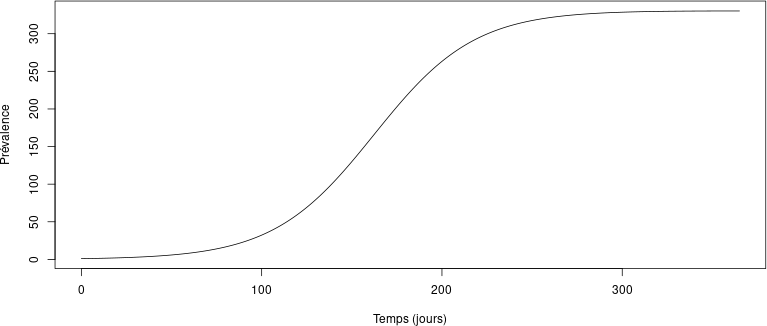
\includegraphics[width=\textwidth]{FIGS/sol_endemic_SIS_R015.png}
  \end{center}
\end{frame}

\begin{frame}{I just did ...}

What I advise not to do: illustrate a mathematical result without adding anything to the result itself
\vfill
Let us make things a bit better. See the \href{https://raw.githubusercontent.com/julien-arino/petit-cours-epidemio-mathematique/main/CODE/ODE_SIS_multiple_solutions.R}{code}
\end{frame}

\begin{frame}{}
  \begin{center}
    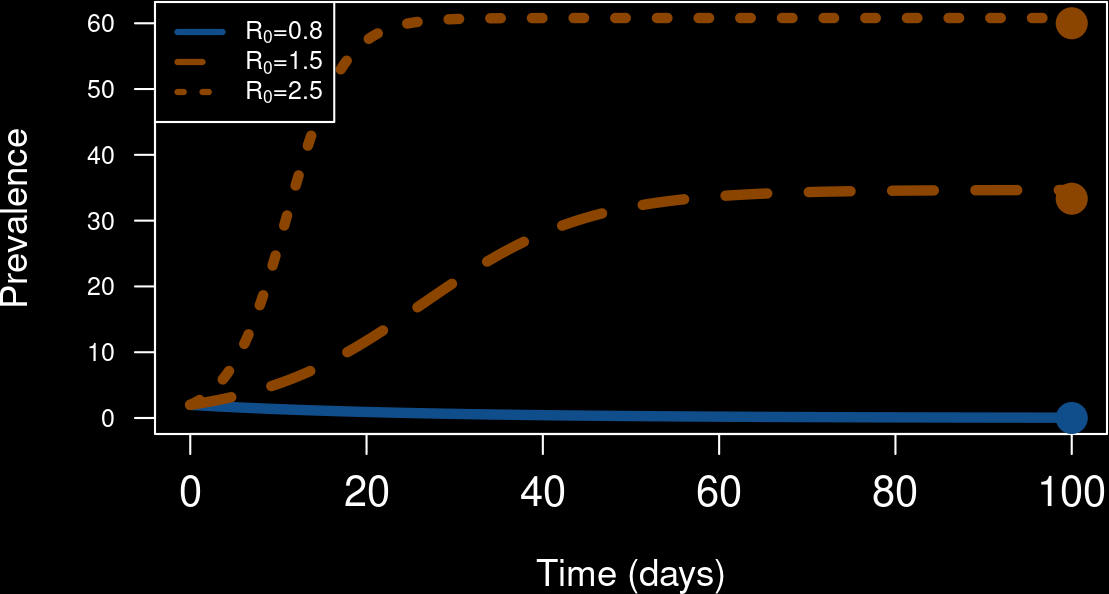
\includegraphics[width=\textwidth]{FIGS/ODE_SIS_multiple_solutions_blackBG.png}
  \end{center}
\end{frame}

\begin{frame}
We could continue, but with a model this simple, there is little  more to do: the 3 parameters of the system are combined within $\R_0$ and the latter summarises the dynamics well
\vfill
We are going to show something important: the bifurcation diagram
\vfill
We saw that when $\R_0<1$, $I\to 0$, whereas when $\R_0>1$, $I\to (1-1/\R_0)N$. Let us represent this (\href{https://raw.githubusercontent.com/julien-arino/petit-cours-epidemio-mathematique/main/CODE/SIS_PEI_vs_R0.R}{code})
\end{frame}

\begin{frame}
  \begin{center}
    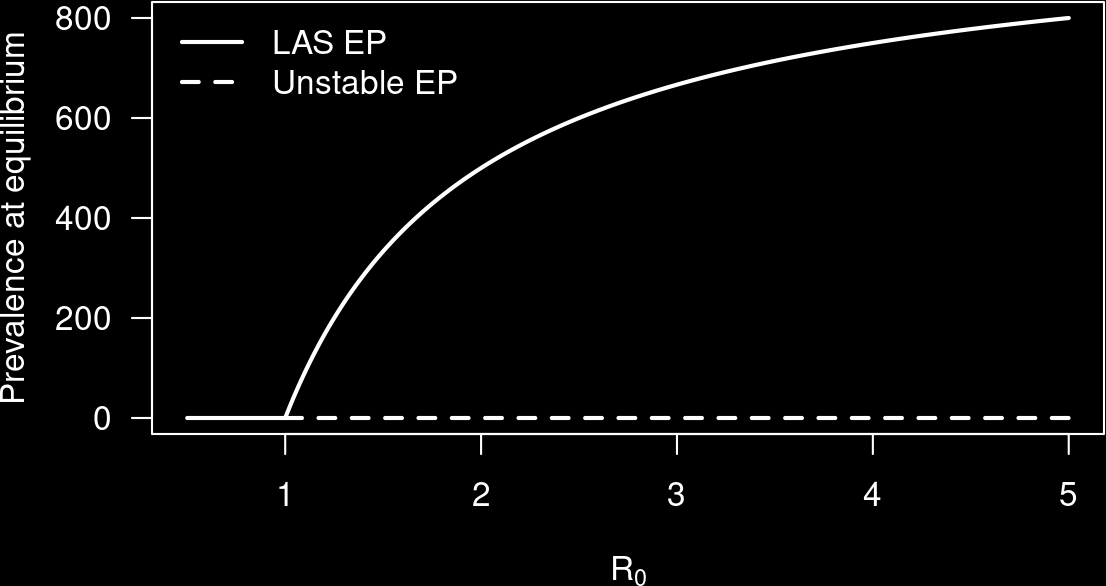
\includegraphics[width=\textwidth]{FIGS/endemic_SIS_EE_vs_R0_blackBG}
  \end{center}
\end{frame}



%%%%%%%%%%%%%%%%%%%%%%%%%%%
%%%%%%%%%%%%%%%%%%%%%%%%%%%
\subsection{An SIR model with vaccination}

\begin{frame}{An SIR model with vaccination}
Take SIRS model \eqref{sys:SIRS} and assume the following
\begin{itemize}
\item Vaccination takes newborn individuals and moves them directly into the removed compartment, without them becoming infected/infectious
\item A fraction $p$ is vaccinated at birth
\end{itemize}
\end{frame}

\begin{frame}{The model}
\begin{minipage}{0.25\textwidth}
  \def\skip{*-1.5}
  \begin{tikzpicture}[scale=1, transform shape]
    %% Regular nodes
    \node [circle, fill=green!50, text=black] at (0,0) (S) {$S$};
    \node [circle, fill=red!90, text=black] at (0,1\skip) (I) {$I$};
    \node [circle, fill=blue!90, text=black] at (0,2\skip) (R) {$R$};
    %% Fake nodes for arrows
    \node [above=1cm of S] (birthS) {};
    \node [below=1cm of R] (birthR) {};
    \node [left=0.5cm of S] (dS) {};
    \node [left=0.5cm of I] (dI) {};
    \node [left=0.5cm of R] (dR) {};
    %% Flows
    \path [line, very thick, red] (birthS) to node [midway, right] (TextNode) {$(1-p)b$} (S);
    \path [line, very thick, red] (birthR) to node [midway, right] (TextNode) {$pb$} (R);
    \path [line, very thick] (S) to node [midway, above] (TextNode) {$dS$} (dS);
    \path [line, very thick] (I) to node [midway, above] (TextNode) {$dI$} (dI);
    \path [line, very thick] (R) to node [midway, above] (TextNode) {$dR$} (dR);
    \path [line, very thick] (S) to node [midway, right] (TextNode) {$\beta SI$} (I);
    \path [line, very thick] (I) to node [midway, right] (TextNode) {$\gamma I$} (R);
    \draw [>=latex,->, thick, rounded corners] (R) -- (0.8,2\skip) -- (0.8,0) node[midway, right] {$\nu R$} -- (S);
    \end{tikzpicture}    
\end{minipage}
\begin{minipage}{0.7\textwidth}
  \begin{subequations} \label{sys:SIR_vacc}
  \begin{align}
    S' &= (1-p)b+\nu R-dS-\beta SI \label{sys:SIR_vacc_dS} \\
    I' &= \beta SI-(d+\gamma) I \label{sys:SIR_vacc_dI} \\
    R' &= bp+\gamma I-(d+\nu)R \label{sys:SIR_vacc_dR}
  \end{align}    
  \end{subequations}
  \vskip1cm
  Consider the initial value problem consisting in \eqref{sys:SIR_vacc} to which we couple initial conditions $S(0)=S_0\geq 0$, $I(0)=I_0\geq 0$ and $R(0)=R_0\geq 0$
  \vskip1cm
  Typically, we assume $N_0=S_0+I_0+R_0>0$ to avoid a trivial case
  \end{minipage}
\end{frame}

\begin{frame}{This modification doesn't change much}
Equation \eqref{eq:total_pop_general} for the total population is unchanged
\vfill
The Jacobian \eqref{eq:SIRS_Jacobian} at arbitrary point is also unchanged
\vfill 
The DFE is affected, though; as a consequence, so is the reproduction number
\end{frame}

\begin{frame}{The DFE for the SIRS vaccination model}
Considering \eqref{sys:SIR_vacc} at equilibrium and substituting $I^\star=0$ into this system gives
\begin{align*}
0 &= (1-p)b+\nu R^\star-dS^\star \\
0 &= bp-(d+\nu)R^\star
\end{align*}
which we rewrite as the linear system
\[
\begin{pmatrix}
d & -\nu \\ 0 & d+\nu
\end{pmatrix}
\begin{pmatrix}
S^\star \\ R^\star
\end{pmatrix}
=
\begin{pmatrix}
(1-p)b \\ bp
\end{pmatrix}
\]
Thus
\begin{align*}
\begin{pmatrix}
S^\star \\ R^\star
\end{pmatrix}
&= \frac{1}{d(d+\nu)}
\begin{pmatrix}
d+\nu & \nu \\ 0 & d
\end{pmatrix}
\begin{pmatrix}
(1-p)b \\ pb
\end{pmatrix} \\
&= \frac{1}{d(d+\nu)}
\begin{pmatrix}
(d+\nu)(1-p)b+pb\nu \\ pbd
\end{pmatrix}
\end{align*}
\end{frame}

\begin{frame}
As a consequence, the DFE takes the form
\begin{equation}\label{eq:SIRS_vacc_DFE}
E_0^v := (S^\star,I^\star,R^\star) =
\left(
\left(1-p+\frac{p\nu}{d+\nu}\right)N^\star,0,
\frac{pd}{d+\nu}N^\star
\right)
\end{equation}
\vfill
Substituting \eqref{eq:SIRS_vacc_DFE} into the eigenvalue that determines stability of the DFE, $\beta S^\star-(d+\gamma)$, we get
\begin{align*}
\beta S^\star-(d+\gamma)<0 &\iff
\frac\beta{d+\gamma} S^\star <1 \\
&\iff 
\frac\beta{d+\gamma}
\left(1-p+\frac{p\nu}{d+\nu}\right)N^\star<1
\end{align*}
So we define
\begin{equation}\label{eq:SIRS_vacc_R0}
\R_0^v =
\frac\beta{d+\gamma}
\left(1-p+\frac{p\nu}{d+\nu}\right)N^\star
\end{equation}
\end{frame}


\begin{frame}{Herd immunity}
  Therefore 
  - $\R_0^{\textrm{v}}<\R_0$ if $p>0$
  - To control the disease, $\R_0^{\text{v}}$ must take a value less than 1, i.e.,
  \begin{equation}
    \R_0^{\text{v}}<1 \iff p> 1-\frac{1}{\R_0}
  \end{equation}
  \vfill
  By vaccinating a fraction $p>1-1/\R_0$ of newborns, we thus are in a situation where the disease is eventually eradicated
  \vfill
  This is \defword{herd immunity}
\end{frame}


%%%%%%%%%%%%%%%%%%%%%%%%%%%
%%%%%%%%%%%%%%%%%%%%%%%%%%%
%%%%%%%%%%%%%%%%%%%%%%%%%%%
%%%%%%%%%%%%%%%%%%%%%%%%%%%
\section{Last remarks}

\begin{frame}{To simplify or not to simplify?}
\bbullet In the KMK epidemic model \eqref{sys:KMK} and the SIRS endemic model \eqref{sys:SIRS}, since the total population is constant or asymptotically constant, it is possible to omit one of the state variables since $N^\star=S+I+R$
\vfill
\bbullet We often use $R=N^\star-S-I$
\vfill
\bbullet This can greatly simplify some computations
\vfill
\bbullet Whether to do it or not is a matter of preference
\end{frame}

\begin{frame}{To normalise or not to normalise?}
\bbullet In the KMK epidemic model \eqref{sys:KMK} and the SIRS endemic model \eqref{sys:SIRS}, since the total population is constant or asymptotically constant, it is possible to normalise to $N=1$
\vfill
\bbullet This can greatly simplify some computations
\vfill
\bbullet However, I am not a big fan: it is important to always have the ``sizes'' of objects in mind
\vfill
\bbullet If you do normalise, at least for a paper destined to mathematical biology, always do a ``return to biology'', i.e., interpret your results in a biological light, which often implies to return to original values
\end{frame}

\begin{frame}{Where we are}
\bbullet An \emph{epidemic} SIR model (the KMK SIR) in which the presence or absence of an epidemic wave is characterised by the value of $\R_0$
\vfill
\bbullet The KMK SIR has explicit solutions (in some sense). \textbf{This is an exception!}
\vfill
\bbullet An \emph{endemic} SIRS model in which the threshold $\R_0=1$ is such that, when $\R_0<1$, the disease goes extinct, whereas when $\R_0>1$, the disease becomes established in the population
\end{frame}



\end{document}
